\documentclass[a4paper]{book}
\usepackage{a4wide}
\usepackage{makeidx}
\usepackage{graphicx}
\usepackage{multicol}
\usepackage{float}
\usepackage{listings}
\usepackage{color}
\usepackage{textcomp}
\usepackage{alltt}
\usepackage{times}
\usepackage{ifpdf}
\ifpdf
\usepackage[pdftex,
            pagebackref=true,
            colorlinks=true,
            linkcolor=blue,
            unicode
           ]{hyperref}
\else
\usepackage[ps2pdf,
            pagebackref=true,
            colorlinks=true,
            linkcolor=blue,
            unicode
           ]{hyperref}
\usepackage{pspicture}
\fi
\usepackage[utf8]{inputenc}
\usepackage[french]{babel}

\usepackage{doxygen}
\lstset{language=C++,inputencoding=utf8,basicstyle=\footnotesize,breaklines=true,breakatwhitespace=true,tabsize=8,numbers=left }
\makeindex
\setcounter{tocdepth}{3}
\renewcommand{\footrulewidth}{0.4pt}
\begin{document}
\hypersetup{pageanchor=false}
\begin{titlepage}
\vspace*{7cm}
\begin{center}
{\Large ProjetSTR-\/Tramway }\\
\vspace*{1cm}
{\large Généré par Doxygen 1.6.3}\\
\vspace*{0.5cm}
{\small Fri Apr 1 09:26:35 2011}\\
\end{center}
\end{titlepage}
\clearemptydoublepage
\pagenumbering{roman}
\tableofcontents
\clearemptydoublepage
\pagenumbering{arabic}
\hypersetup{pageanchor=true}
\chapter{Index des classes}
\section{Hiérarchie des classes}
Cette liste d'héritage est classée approximativement par ordre alphabétique :\begin{DoxyCompactList}
\item \contentsline{section}{Ligne}{\pageref{classLigne}}{}
\item \contentsline{section}{MainWindow}{\pageref{classMainWindow}}{}
\item \contentsline{section}{Passager}{\pageref{classPassager}}{}
\item \contentsline{section}{Signals}{\pageref{classSignals}}{}
\item \contentsline{section}{Thread}{\pageref{classThread}}{}
\begin{DoxyCompactList}
\item \contentsline{section}{GestionSignal}{\pageref{classGestionSignal}}{}
\begin{DoxyCompactList}
\item \contentsline{section}{Element}{\pageref{classElement}}{}
\begin{DoxyCompactList}
\item \contentsline{section}{Obstacle}{\pageref{classObstacle}}{}
\item \contentsline{section}{PointSynchronisation}{\pageref{classPointSynchronisation}}{}
\begin{DoxyCompactList}
\item \contentsline{section}{Feux}{\pageref{classFeux}}{}
\item \contentsline{section}{Station}{\pageref{classStation}}{}
\end{DoxyCompactList}
\end{DoxyCompactList}
\item \contentsline{section}{Porte}{\pageref{classPorte}}{}
\item \contentsline{section}{Rame}{\pageref{classRame}}{}
\end{DoxyCompactList}
\end{DoxyCompactList}
\end{DoxyCompactList}

\chapter{Index des classes}
\section{Liste des classes}
Liste des classes, structures, unions et interfaces avec une brève description :\begin{DoxyCompactList}
\item\contentsline{section}{\hyperlink{classElement}{Element} }{\pageref{classElement}}{}
\item\contentsline{section}{\hyperlink{classFeux}{Feux} }{\pageref{classFeux}}{}
\item\contentsline{section}{\hyperlink{classGestionSignal}{GestionSignal} }{\pageref{classGestionSignal}}{}
\item\contentsline{section}{\hyperlink{classLigne}{Ligne} }{\pageref{classLigne}}{}
\item\contentsline{section}{\hyperlink{classMainWindow}{MainWindow} }{\pageref{classMainWindow}}{}
\item\contentsline{section}{\hyperlink{classObstacle}{Obstacle} }{\pageref{classObstacle}}{}
\item\contentsline{section}{\hyperlink{classPassager}{Passager} }{\pageref{classPassager}}{}
\item\contentsline{section}{\hyperlink{classPointSynchronisation}{PointSynchronisation} }{\pageref{classPointSynchronisation}}{}
\item\contentsline{section}{\hyperlink{classPorte}{Porte} }{\pageref{classPorte}}{}
\item\contentsline{section}{\hyperlink{classRame}{Rame} }{\pageref{classRame}}{}
\item\contentsline{section}{\hyperlink{classSignals}{Signals} }{\pageref{classSignals}}{}
\item\contentsline{section}{\hyperlink{classStation}{Station} }{\pageref{classStation}}{}
\item\contentsline{section}{\hyperlink{classThread}{Thread} }{\pageref{classThread}}{}
\end{DoxyCompactList}

\chapter{Documentation des classes}
\hypertarget{classElement}{
\section{Référence de la classe Element}
\label{classElement}\index{Element@{Element}}
}
Graphe d'héritage de Element:\begin{figure}[H]
\begin{center}
\leavevmode
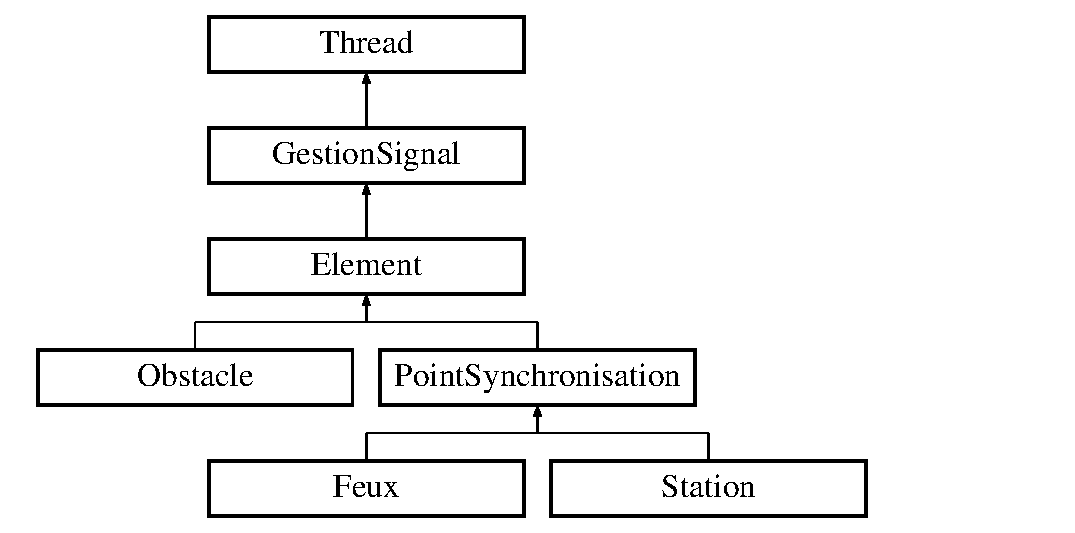
\includegraphics[height=5cm]{classElement}
\end{center}
\end{figure}
\subsection*{Fonctions membres publiques}
\begin{DoxyCompactItemize}
\item 
\hypertarget{classElement_ab0d0e20be9a36ae676202db753faeec9}{
\hyperlink{classElement_ab0d0e20be9a36ae676202db753faeec9}{Element} ()}
\label{classElement_ab0d0e20be9a36ae676202db753faeec9}

\begin{DoxyCompactList}\small\item\em Constructeur de \hyperlink{classElement}{Element}. \item\end{DoxyCompactList}\item 
virtual void \hyperlink{classElement_aabcc968ccfa004f84bddda789441368b}{afficher} (QPainter $\ast$painter, int x, int y, int, int)
\begin{DoxyCompactList}\small\item\em Affichage graphique d'un element. \item\end{DoxyCompactList}\item 
\hypertarget{classElement_a4f4cc97e3122305ec6f4a8953aba23d5}{
virtual void \hyperlink{classElement_a4f4cc97e3122305ec6f4a8953aba23d5}{createSignal} ()}
\label{classElement_a4f4cc97e3122305ec6f4a8953aba23d5}

\begin{DoxyCompactList}\small\item\em Traitement des signaux reçus. \item\end{DoxyCompactList}\end{DoxyCompactItemize}


\subsection{Documentation des fonctions membres}
\hypertarget{classElement_aabcc968ccfa004f84bddda789441368b}{
\index{Element@{Element}!afficher@{afficher}}
\index{afficher@{afficher}!Element@{Element}}
\subsubsection[{afficher}]{\setlength{\rightskip}{0pt plus 5cm}void Element::afficher (QPainter $\ast$ {\em painter}, \/  int {\em x}, \/  int {\em y}, \/  int {\em wElement}, \/  int {\em hElement})\hspace{0.3cm}{\ttfamily  \mbox{[}virtual\mbox{]}}}}
\label{classElement_aabcc968ccfa004f84bddda789441368b}


Affichage graphique d'un element. 


\begin{DoxyParams}{Paramètres}
\item[{\em }]\end{DoxyParams}


Réimplémentée dans \hyperlink{classFeux_a8bb7f9817c38d79927c9a4b471534889}{Feux}, \hyperlink{classObstacle_a77cfc135a2b1fdfe4fab6c7c3713a749}{Obstacle}, et \hyperlink{classPointSynchronisation_a53db6636fdb405bb30fab20b7dc4d374}{PointSynchronisation}.



La documentation de cette classe a été générée à partir des fichiers suivants :\begin{DoxyCompactItemize}
\item 
element.h\item 
element.cpp\end{DoxyCompactItemize}

\hypertarget{classFeux}{
\section{Référence de la classe Feux}
\label{classFeux}\index{Feux@{Feux}}
}
Graphe d'héritage de Feux:\begin{figure}[H]
\begin{center}
\leavevmode
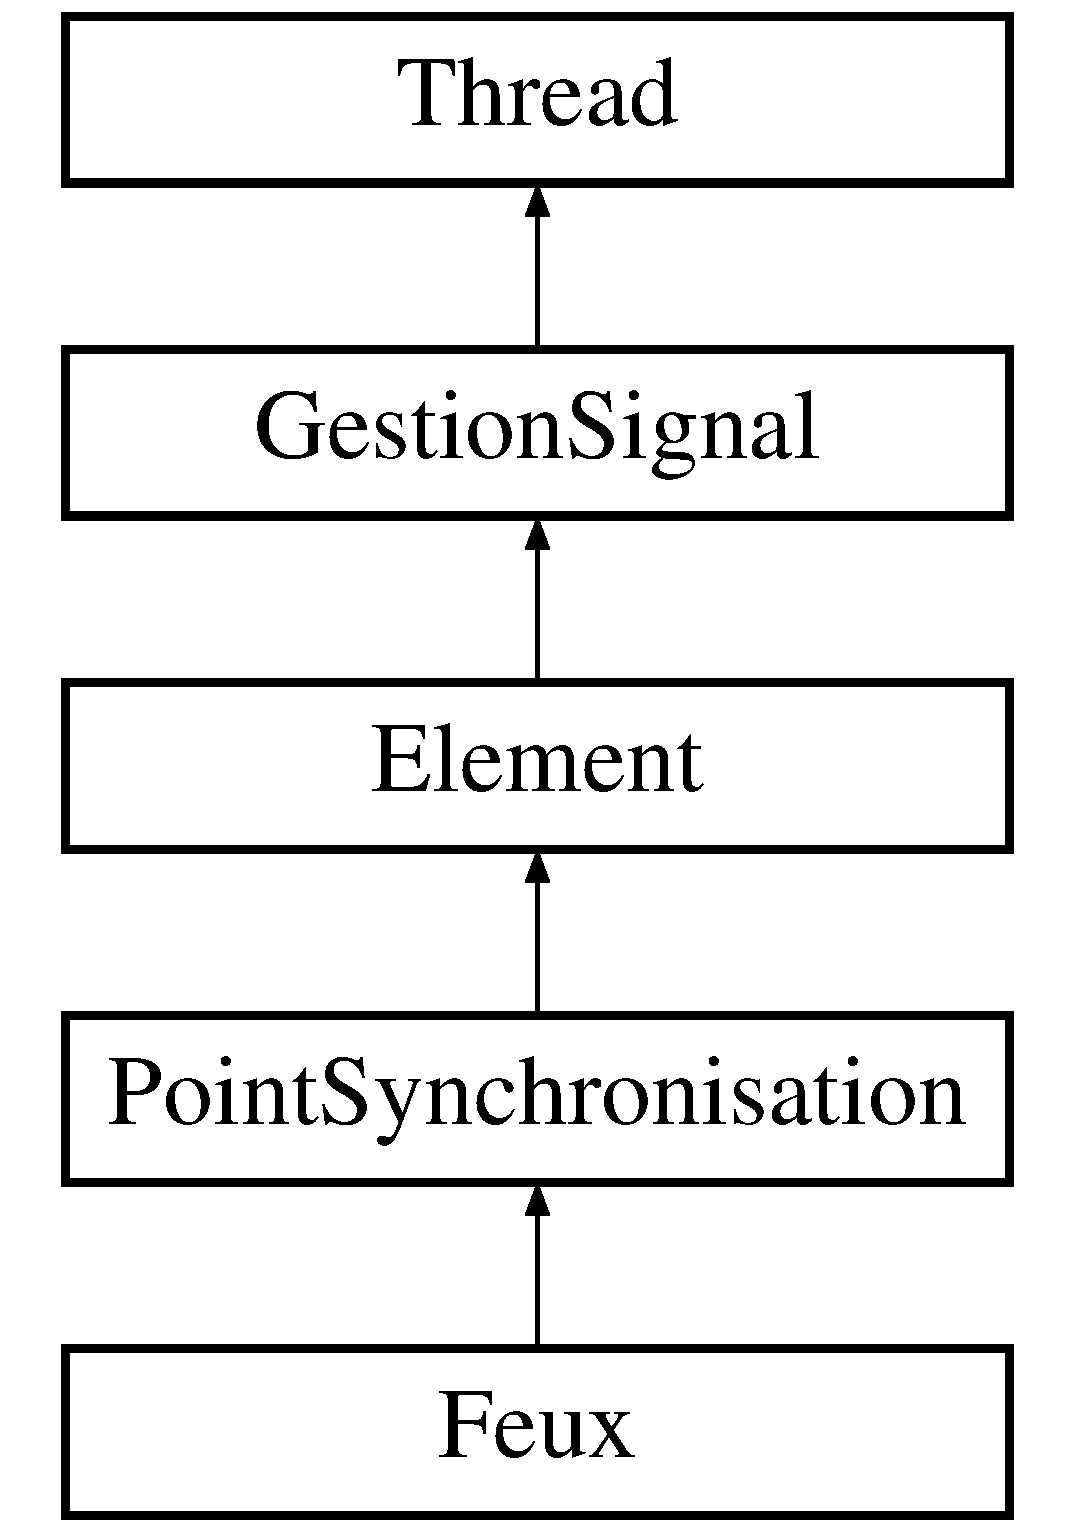
\includegraphics[height=5cm]{classFeux}
\end{center}
\end{figure}
\subsection*{Fonctions membres publiques}
\begin{DoxyCompactItemize}
\item 
\hypertarget{classFeux_a2474d3dc42d3a0d60427f0d2ccf2472e}{
\hyperlink{classFeux_a2474d3dc42d3a0d60427f0d2ccf2472e}{Feux} ()}
\label{classFeux_a2474d3dc42d3a0d60427f0d2ccf2472e}

\begin{DoxyCompactList}\small\item\em constructeur de Feu. \item\end{DoxyCompactList}\item 
\hyperlink{classFeux_a875eac84cbac9d6ea9f2505cb59b0701}{Feux} (\hyperlink{classLigne}{Ligne} $\ast$)
\begin{DoxyCompactList}\small\item\em Constructeur de Feu. \item\end{DoxyCompactList}\item 
\hypertarget{classFeux_a83d13185bdc10129517185ac9579339b}{
\hyperlink{classFeux_a83d13185bdc10129517185ac9579339b}{$\sim$Feux} ()}
\label{classFeux_a83d13185bdc10129517185ac9579339b}

\begin{DoxyCompactList}\small\item\em Destructeur de Feu. \item\end{DoxyCompactList}\item 
\hypertarget{classFeux_a5a868ea5221a779cd2334f892dba0241}{
void \hyperlink{classFeux_a5a868ea5221a779cd2334f892dba0241}{run} ()}
\label{classFeux_a5a868ea5221a779cd2334f892dba0241}

\begin{DoxyCompactList}\small\item\em Comportement d'un feu. \item\end{DoxyCompactList}\item 
virtual void \hyperlink{classFeux_a8bb7f9817c38d79927c9a4b471534889}{afficher} (QPainter $\ast$painter, int x, int y, int, int)
\begin{DoxyCompactList}\small\item\em Affichage graphique d'un feu. \item\end{DoxyCompactList}\item 
virtual QString \hyperlink{classFeux_ac06b420ea2bb015007eb03ca2401176e}{getClasse} ()
\begin{DoxyCompactList}\small\item\em Retourne le nom de la classe Feu. \item\end{DoxyCompactList}\item 
\hypertarget{classFeux_af8488543d58945794535cca3ce9017a0}{
void \hyperlink{classFeux_af8488543d58945794535cca3ce9017a0}{createSignal} ()}
\label{classFeux_af8488543d58945794535cca3ce9017a0}

\begin{DoxyCompactList}\small\item\em Traitement des signaux reçus. \item\end{DoxyCompactList}\end{DoxyCompactItemize}
\subsection*{Attributs publics statiques}
\begin{DoxyCompactItemize}
\item 
\hypertarget{classFeux_a8116829495e0871822c38ed26f09383f}{
static int {\bfseries nombreFeux} = 0}
\label{classFeux_a8116829495e0871822c38ed26f09383f}

\end{DoxyCompactItemize}


\subsection{Documentation des constructeurs et destructeur}
\hypertarget{classFeux_a875eac84cbac9d6ea9f2505cb59b0701}{
\index{Feux@{Feux}!Feux@{Feux}}
\index{Feux@{Feux}!Feux@{Feux}}
\subsubsection[{Feux}]{\setlength{\rightskip}{0pt plus 5cm}Feux::Feux ({\bf Ligne} $\ast$ {\em ligne})}}
\label{classFeux_a875eac84cbac9d6ea9f2505cb59b0701}


Constructeur de Feu. 


\begin{DoxyParams}{Paramètres}
\item[{\em une}]ligne \end{DoxyParams}


\subsection{Documentation des fonctions membres}
\hypertarget{classFeux_a8bb7f9817c38d79927c9a4b471534889}{
\index{Feux@{Feux}!afficher@{afficher}}
\index{afficher@{afficher}!Feux@{Feux}}
\subsubsection[{afficher}]{\setlength{\rightskip}{0pt plus 5cm}void Feux::afficher (QPainter $\ast$ {\em painter}, \/  int {\em x}, \/  int {\em y}, \/  int {\em wElement}, \/  int {\em hElement})\hspace{0.3cm}{\ttfamily  \mbox{[}virtual\mbox{]}}}}
\label{classFeux_a8bb7f9817c38d79927c9a4b471534889}


Affichage graphique d'un feu. 


\begin{DoxyParams}{Paramètres}
\item[{\em }]\end{DoxyParams}


Réimplémentée à partir de \hyperlink{classPointSynchronisation_a53db6636fdb405bb30fab20b7dc4d374}{PointSynchronisation}.

\hypertarget{classFeux_ac06b420ea2bb015007eb03ca2401176e}{
\index{Feux@{Feux}!getClasse@{getClasse}}
\index{getClasse@{getClasse}!Feux@{Feux}}
\subsubsection[{getClasse}]{\setlength{\rightskip}{0pt plus 5cm}virtual QString Feux::getClasse ()\hspace{0.3cm}{\ttfamily  \mbox{[}inline, virtual\mbox{]}}}}
\label{classFeux_ac06b420ea2bb015007eb03ca2401176e}


Retourne le nom de la classe Feu. 

\begin{DoxyReturn}{Renvoie}
le nom de la classe 
\end{DoxyReturn}


Réimplémentée à partir de \hyperlink{classThread_ad055e7c603fda2607670f69c32b2d98a}{Thread}.



La documentation de cette classe a été générée à partir des fichiers suivants :\begin{DoxyCompactItemize}
\item 
feux.h\item 
feux.cpp\end{DoxyCompactItemize}

\hypertarget{classGestionSignal}{
\section{Référence de la classe GestionSignal}
\label{classGestionSignal}\index{GestionSignal@{GestionSignal}}
}
Graphe d'héritage de GestionSignal:\begin{figure}[H]
\begin{center}
\leavevmode
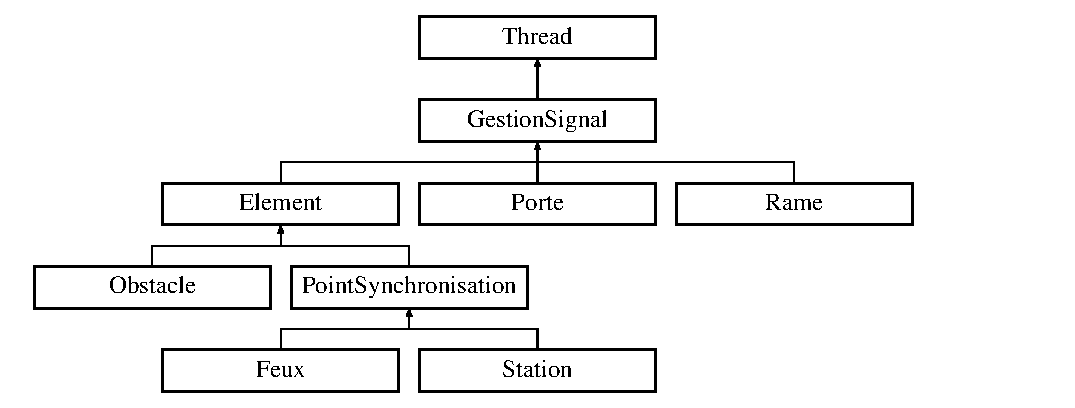
\includegraphics[height=5cm]{classGestionSignal}
\end{center}
\end{figure}
\subsection*{Fonctions membres publiques}
\begin{DoxyCompactItemize}
\item 
\hypertarget{classGestionSignal_af7ab58d9b5971b4b67eec295b76d3b4a}{
\hyperlink{classGestionSignal_af7ab58d9b5971b4b67eec295b76d3b4a}{GestionSignal} ()}
\label{classGestionSignal_af7ab58d9b5971b4b67eec295b76d3b4a}

\begin{DoxyCompactList}\small\item\em Constructeur d'un gestionnaire de signaux. \item\end{DoxyCompactList}\item 
\hypertarget{classGestionSignal_ae28c5d1d8dcda2ff2cd007f89c5d193d}{
\hyperlink{classGestionSignal_ae28c5d1d8dcda2ff2cd007f89c5d193d}{$\sim$GestionSignal} ()}
\label{classGestionSignal_ae28c5d1d8dcda2ff2cd007f89c5d193d}

\begin{DoxyCompactList}\small\item\em Destructeur du gestionnaire de signaux. \item\end{DoxyCompactList}\item 
void \hyperlink{classGestionSignal_a0b729617a3132c6f3227072511ffcb63}{addSignal} (\hyperlink{classSignals}{Signals} $\ast$)
\begin{DoxyCompactList}\small\item\em Ajout d'un signal à la liste de signaux. \item\end{DoxyCompactList}\item 
\hypertarget{classGestionSignal_a4fa2c7af04eaf98de9169709696c1c93}{
virtual void \hyperlink{classGestionSignal_a4fa2c7af04eaf98de9169709696c1c93}{run} ()}
\label{classGestionSignal_a4fa2c7af04eaf98de9169709696c1c93}

\begin{DoxyCompactList}\small\item\em Comportement d'un \hyperlink{classThread}{Thread}. \item\end{DoxyCompactList}\end{DoxyCompactItemize}
\subsection*{Fonctions membres protégées}
\begin{DoxyCompactItemize}
\item 
\hypertarget{classGestionSignal_a1e4fb5f2fa8c0f844639f6bd84ff701b}{
virtual void {\bfseries createSignal} ()=0}
\label{classGestionSignal_a1e4fb5f2fa8c0f844639f6bd84ff701b}

\item 
\hypertarget{classGestionSignal_adf3f0a7f9445d4b81c24aba5adaa89e2}{
void \hyperlink{classGestionSignal_adf3f0a7f9445d4b81c24aba5adaa89e2}{deleteSignal} ()}
\label{classGestionSignal_adf3f0a7f9445d4b81c24aba5adaa89e2}

\begin{DoxyCompactList}\small\item\em Supprime un signal de la liste des signaux. \item\end{DoxyCompactList}\end{DoxyCompactItemize}
\subsection*{Attributs protégés}
\begin{DoxyCompactItemize}
\item 
\hypertarget{classGestionSignal_a6e8cffa17bc2f240d2ab3cdba9b3f53d}{
QList$<$ \hyperlink{classSignals}{Signals} $\ast$ $>$ {\bfseries listSignals}}
\label{classGestionSignal_a6e8cffa17bc2f240d2ab3cdba9b3f53d}

\end{DoxyCompactItemize}


\subsection{Documentation des fonctions membres}
\hypertarget{classGestionSignal_a0b729617a3132c6f3227072511ffcb63}{
\index{GestionSignal@{GestionSignal}!addSignal@{addSignal}}
\index{addSignal@{addSignal}!GestionSignal@{GestionSignal}}
\subsubsection[{addSignal}]{\setlength{\rightskip}{0pt plus 5cm}void GestionSignal::addSignal ({\bf Signals} $\ast$ {\em s})}}
\label{classGestionSignal_a0b729617a3132c6f3227072511ffcb63}


Ajout d'un signal à la liste de signaux. 


\begin{DoxyParams}{Paramètres}
\item[{\em Un}]signal \end{DoxyParams}


La documentation de cette classe a été générée à partir des fichiers suivants :\begin{DoxyCompactItemize}
\item 
gestionsignal.h\item 
gestionsignal.cpp\end{DoxyCompactItemize}

\hypertarget{classLigne}{
\section{Référence de la classe Ligne}
\label{classLigne}\index{Ligne@{Ligne}}
}
\subsection*{Fonctions membres publiques}
\begin{DoxyCompactItemize}
\item 
\hypertarget{classLigne_aa8953c4b617add4054ed9f73b36995b7}{
\hyperlink{classLigne_aa8953c4b617add4054ed9f73b36995b7}{Ligne} ()}
\label{classLigne_aa8953c4b617add4054ed9f73b36995b7}

\begin{DoxyCompactList}\small\item\em Constructeur d'une ligne. \item\end{DoxyCompactList}\item 
\hyperlink{classLigne_a4c5b5e8f49c5b37724685e2c4799fa60}{Ligne} (int longueur)
\begin{DoxyCompactList}\small\item\em Constructeur d'une ligne. \item\end{DoxyCompactList}\item 
\hypertarget{classLigne_a7496e90cf05bab745e3645919d33c811}{
\hyperlink{classLigne_a7496e90cf05bab745e3645919d33c811}{$\sim$Ligne} ()}
\label{classLigne_a7496e90cf05bab745e3645919d33c811}

\begin{DoxyCompactList}\small\item\em Destructeur d'une ligne. \item\end{DoxyCompactList}\item 
void \hyperlink{classLigne_a548b1d11662e76b5bb05a8a4c1bd96de}{afficher} (QPainter $\ast$painter, int, int)
\begin{DoxyCompactList}\small\item\em Affichage graphique d'une ligne. \item\end{DoxyCompactList}\item 
void \hyperlink{classLigne_a4e6647ba0bf16758fecd57d38266c2f0}{ajouterRame} (\hyperlink{classRame}{Rame} $\ast$rame)
\begin{DoxyCompactList}\small\item\em Ajout d'une rame à la ligne. \item\end{DoxyCompactList}\item 
\hypertarget{classLigne_af11dd876c3d78e3fc9a11d0c91eac46f}{
void \hyperlink{classLigne_af11dd876c3d78e3fc9a11d0c91eac46f}{updateListPSsuivant} ()}
\label{classLigne_af11dd876c3d78e3fc9a11d0c91eac46f}

\begin{DoxyCompactList}\small\item\em Definir les objets suivants de chaque points. \item\end{DoxyCompactList}\item 
\hypertarget{classLigne_a58643181ea386f7cc5dd9fa2cd0f00eb}{
void \hyperlink{classLigne_a58643181ea386f7cc5dd9fa2cd0f00eb}{updateListPSprecedent} ()}
\label{classLigne_a58643181ea386f7cc5dd9fa2cd0f00eb}

\begin{DoxyCompactList}\small\item\em Definir les objets precedents de chaque points. \item\end{DoxyCompactList}\item 
\hypertarget{classLigne_a513425699b8fe187f87626923c32c96a}{
void \hyperlink{classLigne_a513425699b8fe187f87626923c32c96a}{ajouterObstacle} ()}
\label{classLigne_a513425699b8fe187f87626923c32c96a}

\begin{DoxyCompactList}\small\item\em Ajouter un obstacle sur la ligne. \item\end{DoxyCompactList}\item 
QList$<$ \hyperlink{classRame}{Rame} $\ast$ $>$ $\ast$ \hyperlink{classLigne_aed26ffc704040dea3ba2b1a8b184a550}{getRames} ()
\begin{DoxyCompactList}\small\item\em Recuperer la liste de rames. \item\end{DoxyCompactList}\item 
\hyperlink{classRame}{Rame} $\ast$ \hyperlink{classLigne_a6c0c5346eff4bc5713241fd4f07fb9ef}{getRameAt} (int)
\begin{DoxyCompactList}\small\item\em Recuperer une rame à une position donnee. \item\end{DoxyCompactList}\item 
int \hyperlink{classLigne_a092ab7c50400c0580c23c9dcf3ba795b}{getLongueur} ()
\begin{DoxyCompactList}\small\item\em Recuperer la longueur de la ligne. \item\end{DoxyCompactList}\item 
int \hyperlink{classLigne_aa48c45c4ab09834ed3ce563985b4955a}{getNbRames} ()
\begin{DoxyCompactList}\small\item\em Recuperer le nombre de rame de la ligne. \item\end{DoxyCompactList}\item 
\hyperlink{classElement}{Element} $\ast$ \hyperlink{classLigne_ad1e50a586085b6d90142cebf0f6b445c}{getElementAt} (int i, bool)
\begin{DoxyCompactList}\small\item\em Recuperer l'element de la position donnee. \item\end{DoxyCompactList}\item 
QList$<$ \hyperlink{classElement}{Element} $\ast$ $>$ $\ast$ \hyperlink{classLigne_a23be9d51e86eac91160cec43bf2edbe0}{getListeElement} ()
\begin{DoxyCompactList}\small\item\em Recuperer la liste des elements de la ligne. \item\end{DoxyCompactList}\item 
QList$<$ \hyperlink{classStation}{Station} $\ast$ $>$ $\ast$ \hyperlink{classLigne_a8ced36e42672723b6e0037c389e59bb4}{getStations} ()
\begin{DoxyCompactList}\small\item\em Recuperer la liste des stations de la ligne. \item\end{DoxyCompactList}\end{DoxyCompactItemize}


\subsection{Documentation des constructeurs et destructeur}
\hypertarget{classLigne_a4c5b5e8f49c5b37724685e2c4799fa60}{
\index{Ligne@{Ligne}!Ligne@{Ligne}}
\index{Ligne@{Ligne}!Ligne@{Ligne}}
\subsubsection[{Ligne}]{\setlength{\rightskip}{0pt plus 5cm}Ligne::Ligne (int {\em longueur})}}
\label{classLigne_a4c5b5e8f49c5b37724685e2c4799fa60}


Constructeur d'une ligne. 


\begin{DoxyParams}{Paramètres}
\item[{\em Longueur}]de la ligne \end{DoxyParams}


\subsection{Documentation des fonctions membres}
\hypertarget{classLigne_a548b1d11662e76b5bb05a8a4c1bd96de}{
\index{Ligne@{Ligne}!afficher@{afficher}}
\index{afficher@{afficher}!Ligne@{Ligne}}
\subsubsection[{afficher}]{\setlength{\rightskip}{0pt plus 5cm}void Ligne::afficher (QPainter $\ast$ {\em painter}, \/  int {\em w}, \/  int {\em h})}}
\label{classLigne_a548b1d11662e76b5bb05a8a4c1bd96de}


Affichage graphique d'une ligne. 


\begin{DoxyParams}{Paramètres}
\item[{\em }]\end{DoxyParams}
\hypertarget{classLigne_a4e6647ba0bf16758fecd57d38266c2f0}{
\index{Ligne@{Ligne}!ajouterRame@{ajouterRame}}
\index{ajouterRame@{ajouterRame}!Ligne@{Ligne}}
\subsubsection[{ajouterRame}]{\setlength{\rightskip}{0pt plus 5cm}void Ligne::ajouterRame ({\bf Rame} $\ast$ {\em rame})}}
\label{classLigne_a4e6647ba0bf16758fecd57d38266c2f0}


Ajout d'une rame à la ligne. 


\begin{DoxyParams}{Paramètres}
\item[{\em }]\end{DoxyParams}
\hypertarget{classLigne_ad1e50a586085b6d90142cebf0f6b445c}{
\index{Ligne@{Ligne}!getElementAt@{getElementAt}}
\index{getElementAt@{getElementAt}!Ligne@{Ligne}}
\subsubsection[{getElementAt}]{\setlength{\rightskip}{0pt plus 5cm}{\bf Element} $\ast$ Ligne::getElementAt (int {\em i}, \/  bool {\em aller})}}
\label{classLigne_ad1e50a586085b6d90142cebf0f6b445c}


Recuperer l'element de la position donnee. 

\begin{DoxyReturn}{Renvoie}
Un element 
\end{DoxyReturn}

\begin{DoxyParams}{Paramètres}
\item[{\em Une}]position \item[{\em ligne}]allee=1 $|$ retour=0 \end{DoxyParams}
\hypertarget{classLigne_a23be9d51e86eac91160cec43bf2edbe0}{
\index{Ligne@{Ligne}!getListeElement@{getListeElement}}
\index{getListeElement@{getListeElement}!Ligne@{Ligne}}
\subsubsection[{getListeElement}]{\setlength{\rightskip}{0pt plus 5cm}QList$<$ {\bf Element} $\ast$ $>$ $\ast$ Ligne::getListeElement ()}}
\label{classLigne_a23be9d51e86eac91160cec43bf2edbe0}


Recuperer la liste des elements de la ligne. 

\begin{DoxyReturn}{Renvoie}
Une liste d'element 
\end{DoxyReturn}
\hypertarget{classLigne_a092ab7c50400c0580c23c9dcf3ba795b}{
\index{Ligne@{Ligne}!getLongueur@{getLongueur}}
\index{getLongueur@{getLongueur}!Ligne@{Ligne}}
\subsubsection[{getLongueur}]{\setlength{\rightskip}{0pt plus 5cm}int Ligne::getLongueur ()}}
\label{classLigne_a092ab7c50400c0580c23c9dcf3ba795b}


Recuperer la longueur de la ligne. 

\begin{DoxyReturn}{Renvoie}
La longueur de la ligne 
\end{DoxyReturn}
\hypertarget{classLigne_aa48c45c4ab09834ed3ce563985b4955a}{
\index{Ligne@{Ligne}!getNbRames@{getNbRames}}
\index{getNbRames@{getNbRames}!Ligne@{Ligne}}
\subsubsection[{getNbRames}]{\setlength{\rightskip}{0pt plus 5cm}int Ligne::getNbRames ()}}
\label{classLigne_aa48c45c4ab09834ed3ce563985b4955a}


Recuperer le nombre de rame de la ligne. 

\begin{DoxyReturn}{Renvoie}
Le nombre de rame 
\end{DoxyReturn}
\hypertarget{classLigne_a6c0c5346eff4bc5713241fd4f07fb9ef}{
\index{Ligne@{Ligne}!getRameAt@{getRameAt}}
\index{getRameAt@{getRameAt}!Ligne@{Ligne}}
\subsubsection[{getRameAt}]{\setlength{\rightskip}{0pt plus 5cm}{\bf Rame} $\ast$ Ligne::getRameAt (int {\em i})}}
\label{classLigne_a6c0c5346eff4bc5713241fd4f07fb9ef}


Recuperer une rame à une position donnee. 


\begin{DoxyParams}{Paramètres}
\item[{\em Position}]sur la ligne \end{DoxyParams}
\hypertarget{classLigne_aed26ffc704040dea3ba2b1a8b184a550}{
\index{Ligne@{Ligne}!getRames@{getRames}}
\index{getRames@{getRames}!Ligne@{Ligne}}
\subsubsection[{getRames}]{\setlength{\rightskip}{0pt plus 5cm}QList$<$ {\bf Rame} $\ast$ $>$ $\ast$ Ligne::getRames ()}}
\label{classLigne_aed26ffc704040dea3ba2b1a8b184a550}


Recuperer la liste de rames. 

\begin{DoxyReturn}{Renvoie}
Une liste de rame 
\end{DoxyReturn}
\hypertarget{classLigne_a8ced36e42672723b6e0037c389e59bb4}{
\index{Ligne@{Ligne}!getStations@{getStations}}
\index{getStations@{getStations}!Ligne@{Ligne}}
\subsubsection[{getStations}]{\setlength{\rightskip}{0pt plus 5cm}QList$<$ {\bf Station} $\ast$ $>$ $\ast$ Ligne::getStations ()}}
\label{classLigne_a8ced36e42672723b6e0037c389e59bb4}


Recuperer la liste des stations de la ligne. 

\begin{DoxyReturn}{Renvoie}
Une liste de station 
\end{DoxyReturn}


La documentation de cette classe a été générée à partir des fichiers suivants :\begin{DoxyCompactItemize}
\item 
ligne.h\item 
ligne.cpp\end{DoxyCompactItemize}

\hypertarget{classMainWindow}{
\section{Référence de la classe MainWindow}
\label{classMainWindow}\index{MainWindow@{MainWindow}}
}
\subsection*{Connecteurs publics}
\begin{DoxyCompactItemize}
\item 
\hypertarget{classMainWindow_af676b5cca5c8975dd3d7d12d70e5ebad}{
void {\bfseries loadTime} ()}
\label{classMainWindow_af676b5cca5c8975dd3d7d12d70e5ebad}

\end{DoxyCompactItemize}
\subsection*{Fonctions membres publiques}
\begin{DoxyCompactItemize}
\item 
\hypertarget{classMainWindow_a8b244be8b7b7db1b08de2a2acb9409db}{
{\bfseries MainWindow} (QWidget $\ast$parent=0)}
\label{classMainWindow_a8b244be8b7b7db1b08de2a2acb9409db}

\item 
\hypertarget{classMainWindow_a37c0b44e6dacc12f4136f4db3ac0cdeb}{
void {\bfseries afficher} ()}
\label{classMainWindow_a37c0b44e6dacc12f4136f4db3ac0cdeb}

\end{DoxyCompactItemize}


La documentation de cette classe a été générée à partir des fichiers suivants :\begin{DoxyCompactItemize}
\item 
mainwindow.h\item 
mainwindow.cpp\end{DoxyCompactItemize}

\hypertarget{classObstacle}{
\section{Référence de la classe Obstacle}
\label{classObstacle}\index{Obstacle@{Obstacle}}
}
Graphe d'héritage de Obstacle:\begin{figure}[H]
\begin{center}
\leavevmode
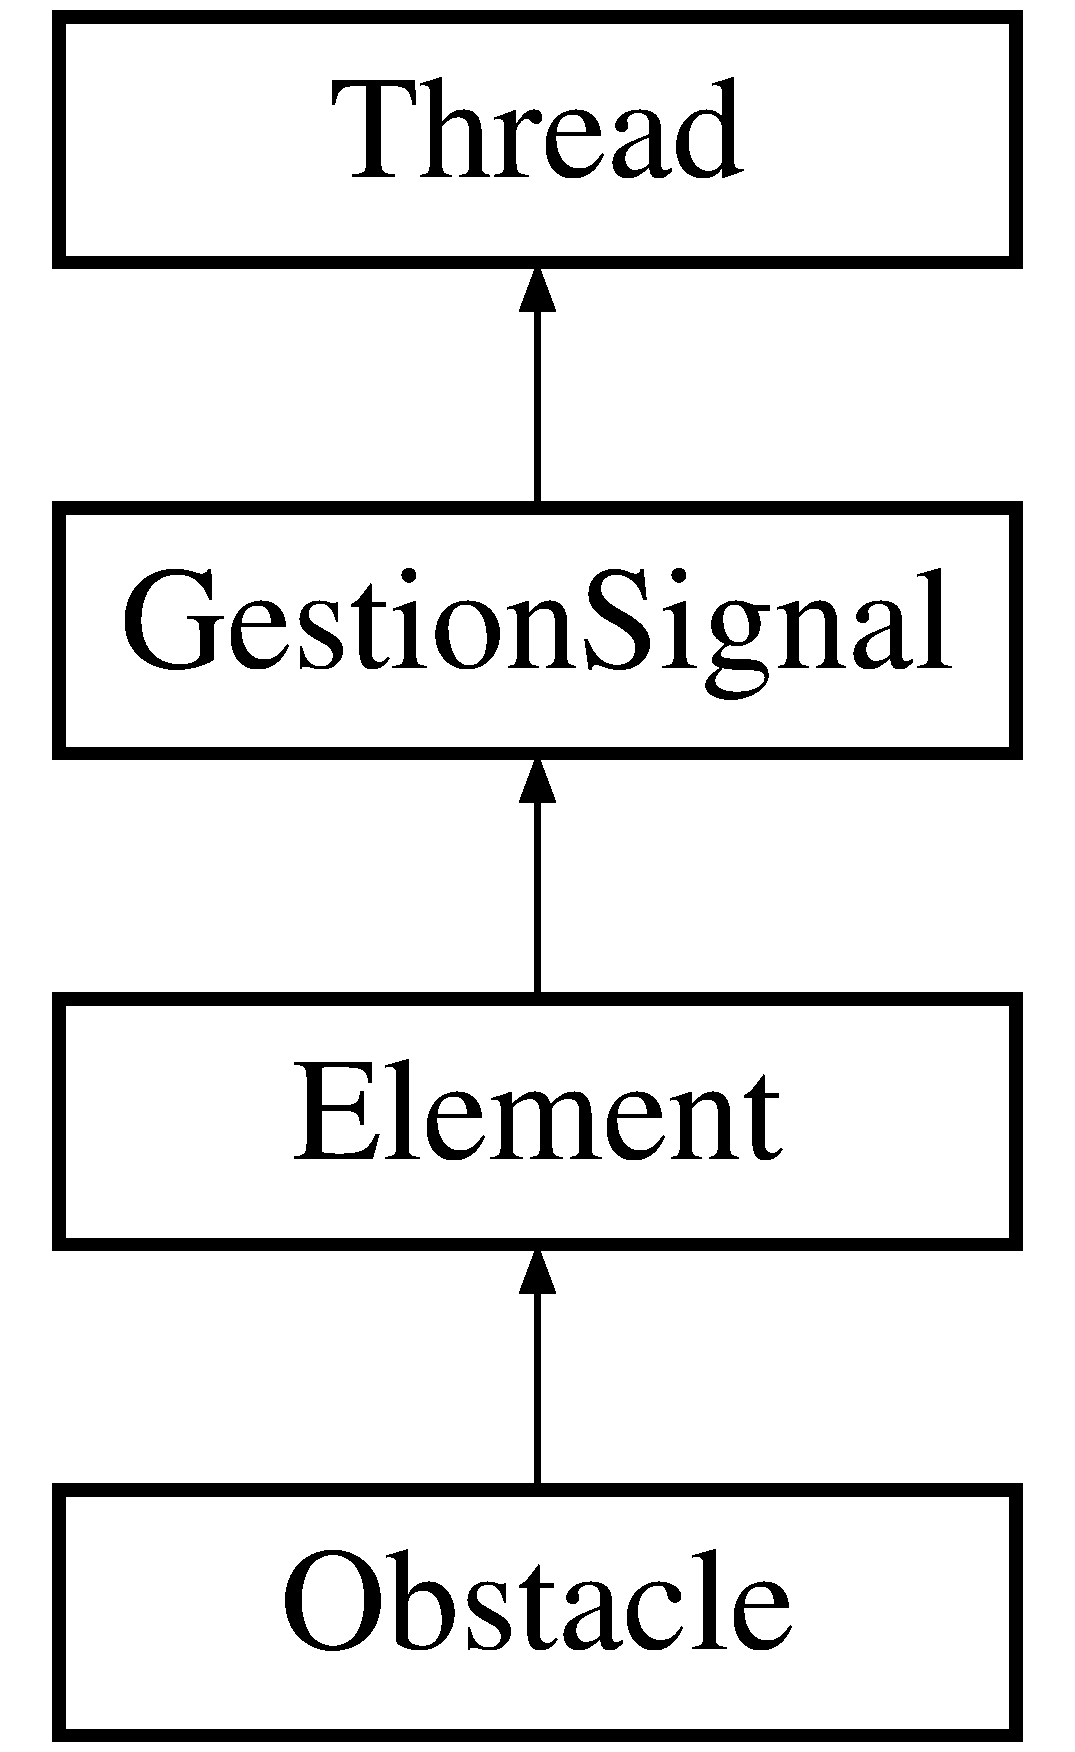
\includegraphics[height=4cm]{classObstacle}
\end{center}
\end{figure}
\subsection*{Fonctions membres publiques}
\begin{DoxyCompactItemize}
\item 
\hypertarget{classObstacle_a8f734072321fa06a7b7dae2d5f50f352}{
\hyperlink{classObstacle_a8f734072321fa06a7b7dae2d5f50f352}{Obstacle} ()}
\label{classObstacle_a8f734072321fa06a7b7dae2d5f50f352}

\begin{DoxyCompactList}\small\item\em Constructeur d'un obstacle. \item\end{DoxyCompactList}\item 
\hyperlink{classObstacle_aaf39f191e411a16f1bd9573da092da04}{Obstacle} (QList$<$ \hyperlink{classElement}{Element} $\ast$ $>$ $\ast$sens, int position)
\begin{DoxyCompactList}\small\item\em Constructeur d'un obstacle. \item\end{DoxyCompactList}\item 
\hypertarget{classObstacle_af2f9cc9c6cff75dca0974fd5ac4f71a9}{
\hyperlink{classObstacle_af2f9cc9c6cff75dca0974fd5ac4f71a9}{$\sim$Obstacle} ()}
\label{classObstacle_af2f9cc9c6cff75dca0974fd5ac4f71a9}

\begin{DoxyCompactList}\small\item\em Destructeur d'obstacle. \item\end{DoxyCompactList}\item 
void \hyperlink{classObstacle_a77cfc135a2b1fdfe4fab6c7c3713a749}{afficher} (QPainter $\ast$painter, int x, int y, int, int)
\begin{DoxyCompactList}\small\item\em Affichage graphique d'une obstacle. \item\end{DoxyCompactList}\item 
QString \hyperlink{classObstacle_a7773466eaafb92cef0ec22f5cc79522c}{getClasse} ()
\begin{DoxyCompactList}\small\item\em Retourne le nom de la classe \hyperlink{classObstacle}{Obstacle}. \item\end{DoxyCompactList}\end{DoxyCompactItemize}


\subsection{Documentation des constructeurs et destructeur}
\hypertarget{classObstacle_aaf39f191e411a16f1bd9573da092da04}{
\index{Obstacle@{Obstacle}!Obstacle@{Obstacle}}
\index{Obstacle@{Obstacle}!Obstacle@{Obstacle}}
\subsubsection[{Obstacle}]{\setlength{\rightskip}{0pt plus 5cm}Obstacle::Obstacle (QList$<$ {\bf Element} $\ast$ $>$ $\ast$ {\em sens}, \/  int {\em position})}}
\label{classObstacle_aaf39f191e411a16f1bd9573da092da04}


Constructeur d'un obstacle. 


\begin{DoxyParams}{Paramètres}
\item[{\em une}]liste d'element \item[{\em la}]position \end{DoxyParams}


\subsection{Documentation des fonctions membres}
\hypertarget{classObstacle_a77cfc135a2b1fdfe4fab6c7c3713a749}{
\index{Obstacle@{Obstacle}!afficher@{afficher}}
\index{afficher@{afficher}!Obstacle@{Obstacle}}
\subsubsection[{afficher}]{\setlength{\rightskip}{0pt plus 5cm}void Obstacle::afficher (QPainter $\ast$ {\em painter}, \/  int {\em x}, \/  int {\em y}, \/  int {\em w}, \/  int {\em h})\hspace{0.3cm}{\ttfamily  \mbox{[}virtual\mbox{]}}}}
\label{classObstacle_a77cfc135a2b1fdfe4fab6c7c3713a749}


Affichage graphique d'une obstacle. 


\begin{DoxyParams}{Paramètres}
\item[{\em }]\end{DoxyParams}


Réimplémentée à partir de \hyperlink{classElement_aabcc968ccfa004f84bddda789441368b}{Element}.

\hypertarget{classObstacle_a7773466eaafb92cef0ec22f5cc79522c}{
\index{Obstacle@{Obstacle}!getClasse@{getClasse}}
\index{getClasse@{getClasse}!Obstacle@{Obstacle}}
\subsubsection[{getClasse}]{\setlength{\rightskip}{0pt plus 5cm}QString Obstacle::getClasse ()\hspace{0.3cm}{\ttfamily  \mbox{[}inline, virtual\mbox{]}}}}
\label{classObstacle_a7773466eaafb92cef0ec22f5cc79522c}


Retourne le nom de la classe \hyperlink{classObstacle}{Obstacle}. 

\begin{DoxyReturn}{Renvoie}
le nom de la classe 
\end{DoxyReturn}


Réimplémentée à partir de \hyperlink{classThread_ad055e7c603fda2607670f69c32b2d98a}{Thread}.



La documentation de cette classe a été générée à partir des fichiers suivants :\begin{DoxyCompactItemize}
\item 
obstacle.h\item 
obstacle.cpp\end{DoxyCompactItemize}

\hypertarget{classPassager}{
\section{Référence de la classe Passager}
\label{classPassager}\index{Passager@{Passager}}
}
\subsection*{Fonctions membres publiques}
\begin{DoxyCompactItemize}
\item 
\hypertarget{classPassager_abaa10f10af62627931cfdf9a57da07e3}{
\hyperlink{classPassager_abaa10f10af62627931cfdf9a57da07e3}{Passager} ()}
\label{classPassager_abaa10f10af62627931cfdf9a57da07e3}

\begin{DoxyCompactList}\small\item\em Constructeur d'un passager. \item\end{DoxyCompactList}\item 
\hyperlink{classPassager_aad5c03eba33134fe3f63bc814b622f2e}{Passager} (\hyperlink{classStation}{Station} $\ast$)
\begin{DoxyCompactList}\small\item\em Constructeur d'un passager. \item\end{DoxyCompactList}\item 
\hypertarget{classPassager_a6afb6fea48617a8eec07a53e7f3f5ebc}{
\hyperlink{classPassager_a6afb6fea48617a8eec07a53e7f3f5ebc}{$\sim$Passager} ()}
\label{classPassager_a6afb6fea48617a8eec07a53e7f3f5ebc}

\begin{DoxyCompactList}\small\item\em Destructeur d'un passager. \item\end{DoxyCompactList}\item 
\hyperlink{classStation}{Station} $\ast$ \hyperlink{classPassager_a743190997fecd1b8b0660c2c93ca4f5f}{getStationDest} ()
\begin{DoxyCompactList}\small\item\em Recuperer la station de destination. \item\end{DoxyCompactList}\end{DoxyCompactItemize}


\subsection{Documentation des constructeurs et destructeur}
\hypertarget{classPassager_aad5c03eba33134fe3f63bc814b622f2e}{
\index{Passager@{Passager}!Passager@{Passager}}
\index{Passager@{Passager}!Passager@{Passager}}
\subsubsection[{Passager}]{\setlength{\rightskip}{0pt plus 5cm}Passager::Passager ({\bf Station} $\ast$ {\em pstatitionDest})}}
\label{classPassager_aad5c03eba33134fe3f63bc814b622f2e}


Constructeur d'un passager. 


\begin{DoxyParams}{Paramètres}
\item[{\em Une}]station \end{DoxyParams}


\subsection{Documentation des fonctions membres}
\hypertarget{classPassager_a743190997fecd1b8b0660c2c93ca4f5f}{
\index{Passager@{Passager}!getStationDest@{getStationDest}}
\index{getStationDest@{getStationDest}!Passager@{Passager}}
\subsubsection[{getStationDest}]{\setlength{\rightskip}{0pt plus 5cm}{\bf Station} $\ast$ Passager::getStationDest ()}}
\label{classPassager_a743190997fecd1b8b0660c2c93ca4f5f}


Recuperer la station de destination. 

\begin{DoxyReturn}{Renvoie}
La station de destination du passager 
\end{DoxyReturn}


La documentation de cette classe a été générée à partir des fichiers suivants :\begin{DoxyCompactItemize}
\item 
passager.h\item 
passager.cpp\end{DoxyCompactItemize}

\hypertarget{classPointSynchronisation}{
\section{Référence de la classe PointSynchronisation}
\label{classPointSynchronisation}\index{PointSynchronisation@{PointSynchronisation}}
}
Graphe d'héritage de PointSynchronisation:\begin{figure}[H]
\begin{center}
\leavevmode
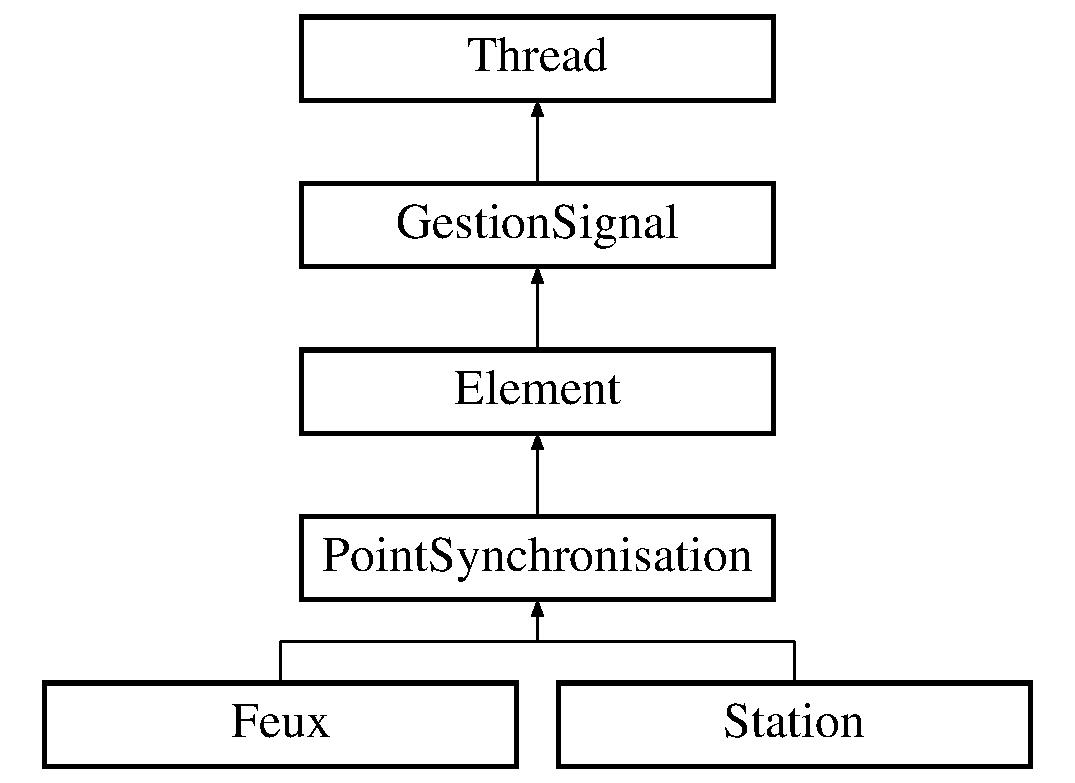
\includegraphics[height=5cm]{classPointSynchronisation}
\end{center}
\end{figure}
\subsection*{Fonctions membres publiques}
\begin{DoxyCompactItemize}
\item 
\hypertarget{classPointSynchronisation_ab0be3460c6b050a8a9a0ff98fc596cb2}{
\hyperlink{classPointSynchronisation_ab0be3460c6b050a8a9a0ff98fc596cb2}{PointSynchronisation} ()}
\label{classPointSynchronisation_ab0be3460c6b050a8a9a0ff98fc596cb2}

\begin{DoxyCompactList}\small\item\em Constructeur d'un point. \item\end{DoxyCompactList}\item 
\hypertarget{classPointSynchronisation_a9ad32b2006c258e3b9b493ae9b67cb49}{
\hyperlink{classPointSynchronisation_a9ad32b2006c258e3b9b493ae9b67cb49}{$\sim$PointSynchronisation} ()}
\label{classPointSynchronisation_a9ad32b2006c258e3b9b493ae9b67cb49}

\begin{DoxyCompactList}\small\item\em Destructeur d'un point de synchronisation. \item\end{DoxyCompactList}\item 
virtual void \hyperlink{classPointSynchronisation_a53db6636fdb405bb30fab20b7dc4d374}{afficher} (QPainter $\ast$painter, int x, int y, int, int)
\begin{DoxyCompactList}\small\item\em Affichage graphique d'un Point. \item\end{DoxyCompactList}\item 
bool \hyperlink{classPointSynchronisation_a230f8d22845e44ea7cd4cb96d9f5128c}{estVert} ()
\begin{DoxyCompactList}\small\item\em Savoir si un point est accessible. \item\end{DoxyCompactList}\item 
\hyperlink{classGestionSignal}{GestionSignal} $\ast$ \hyperlink{classPointSynchronisation_a6cecce4b7274aabe549c96b2d55b0cda}{getDerniereRame} ()
\begin{DoxyCompactList}\small\item\em Recuperer la la derniere rame. \item\end{DoxyCompactList}\item 
\hypertarget{classPointSynchronisation_ac66ba2db21a7120b143b85301680e439}{
void \hyperlink{classPointSynchronisation_ac66ba2db21a7120b143b85301680e439}{passerRouge} ()}
\label{classPointSynchronisation_ac66ba2db21a7120b143b85301680e439}

\begin{DoxyCompactList}\small\item\em Definir un point comme inaccessible. \item\end{DoxyCompactList}\item 
\hypertarget{classPointSynchronisation_a2044b3c16c50491cababb1ff16f03252}{
void \hyperlink{classPointSynchronisation_a2044b3c16c50491cababb1ff16f03252}{passerVert} ()}
\label{classPointSynchronisation_a2044b3c16c50491cababb1ff16f03252}

\begin{DoxyCompactList}\small\item\em Definir un point comme accessible. \item\end{DoxyCompactList}\item 
void \hyperlink{classPointSynchronisation_a8f677010a6ec932eba3b15a586c575ad}{setSuivant} (\hyperlink{classPointSynchronisation}{PointSynchronisation} $\ast$)
\begin{DoxyCompactList}\small\item\em Definir le point suivant. \item\end{DoxyCompactList}\item 
\hyperlink{classPointSynchronisation}{PointSynchronisation} $\ast$ \hyperlink{classPointSynchronisation_a0e5b8f12043e94e9bf5b4a1d798830ff}{getSuivant} ()
\begin{DoxyCompactList}\small\item\em Recuperer le point suivant. \item\end{DoxyCompactList}\item 
void \hyperlink{classPointSynchronisation_a91a058d0174071f36d6132b3afcafdc3}{setPrecedent} (\hyperlink{classPointSynchronisation}{PointSynchronisation} $\ast$)
\begin{DoxyCompactList}\small\item\em Definir le point precedent. \item\end{DoxyCompactList}\item 
\hyperlink{classPointSynchronisation}{PointSynchronisation} $\ast$ \hyperlink{classPointSynchronisation_a7929df6ad2b116b1831c18561000f1bd}{getPrecedent} ()
\begin{DoxyCompactList}\small\item\em Recuperer le point precedent. \item\end{DoxyCompactList}\item 
int \hyperlink{classPointSynchronisation_a46838a33d790814c14cf284f48beac7c}{getNum} ()
\begin{DoxyCompactList}\small\item\em Recuperer le numero du point courant. \item\end{DoxyCompactList}\end{DoxyCompactItemize}
\subsection*{Attributs protégés}
\begin{DoxyCompactItemize}
\item 
\hypertarget{classPointSynchronisation_a1494c8728bfcd6947d6d2583dd61b218}{
bool {\bfseries vert}}
\label{classPointSynchronisation_a1494c8728bfcd6947d6d2583dd61b218}

\item 
\hypertarget{classPointSynchronisation_a42b671076eb43c988b2633783bc6edc0}{
int {\bfseries numPS}}
\label{classPointSynchronisation_a42b671076eb43c988b2633783bc6edc0}

\item 
\hypertarget{classPointSynchronisation_a850786ba609b118d5c18c84ba02be812}{
\hyperlink{classGestionSignal}{GestionSignal} $\ast$ {\bfseries derniereRame}}
\label{classPointSynchronisation_a850786ba609b118d5c18c84ba02be812}

\item 
\hypertarget{classPointSynchronisation_a280e3fc198958636a6b3f4a2d4e12a06}{
\hyperlink{classPointSynchronisation}{PointSynchronisation} $\ast$ {\bfseries suivant}}
\label{classPointSynchronisation_a280e3fc198958636a6b3f4a2d4e12a06}

\item 
\hypertarget{classPointSynchronisation_a813f00f17c496027811f2275a97964cf}{
\hyperlink{classPointSynchronisation}{PointSynchronisation} $\ast$ {\bfseries precedent}}
\label{classPointSynchronisation_a813f00f17c496027811f2275a97964cf}

\end{DoxyCompactItemize}


\subsection{Documentation des fonctions membres}
\hypertarget{classPointSynchronisation_a53db6636fdb405bb30fab20b7dc4d374}{
\index{PointSynchronisation@{PointSynchronisation}!afficher@{afficher}}
\index{afficher@{afficher}!PointSynchronisation@{PointSynchronisation}}
\subsubsection[{afficher}]{\setlength{\rightskip}{0pt plus 5cm}void PointSynchronisation::afficher (QPainter $\ast$ {\em painter}, \/  int {\em x}, \/  int {\em y}, \/  int {\em x1}, \/  int {\em x2})\hspace{0.3cm}{\ttfamily  \mbox{[}virtual\mbox{]}}}}
\label{classPointSynchronisation_a53db6636fdb405bb30fab20b7dc4d374}


Affichage graphique d'un Point. 


\begin{DoxyParams}{Paramètres}
\item[{\em }]\end{DoxyParams}


Réimplémentée à partir de \hyperlink{classElement_aabcc968ccfa004f84bddda789441368b}{Element}.



Réimplémentée dans \hyperlink{classFeux_a8bb7f9817c38d79927c9a4b471534889}{Feux}.

\hypertarget{classPointSynchronisation_a230f8d22845e44ea7cd4cb96d9f5128c}{
\index{PointSynchronisation@{PointSynchronisation}!estVert@{estVert}}
\index{estVert@{estVert}!PointSynchronisation@{PointSynchronisation}}
\subsubsection[{estVert}]{\setlength{\rightskip}{0pt plus 5cm}bool PointSynchronisation::estVert ()}}
\label{classPointSynchronisation_a230f8d22845e44ea7cd4cb96d9f5128c}


Savoir si un point est accessible. 

\begin{DoxyReturn}{Renvoie}
l'etat du point 
\end{DoxyReturn}
\hypertarget{classPointSynchronisation_a6cecce4b7274aabe549c96b2d55b0cda}{
\index{PointSynchronisation@{PointSynchronisation}!getDerniereRame@{getDerniereRame}}
\index{getDerniereRame@{getDerniereRame}!PointSynchronisation@{PointSynchronisation}}
\subsubsection[{getDerniereRame}]{\setlength{\rightskip}{0pt plus 5cm}{\bf GestionSignal} $\ast$ PointSynchronisation::getDerniereRame ()}}
\label{classPointSynchronisation_a6cecce4b7274aabe549c96b2d55b0cda}


Recuperer la la derniere rame. 

\begin{DoxyReturn}{Renvoie}
Une liste de station 
\end{DoxyReturn}
\hypertarget{classPointSynchronisation_a46838a33d790814c14cf284f48beac7c}{
\index{PointSynchronisation@{PointSynchronisation}!getNum@{getNum}}
\index{getNum@{getNum}!PointSynchronisation@{PointSynchronisation}}
\subsubsection[{getNum}]{\setlength{\rightskip}{0pt plus 5cm}int PointSynchronisation::getNum ()}}
\label{classPointSynchronisation_a46838a33d790814c14cf284f48beac7c}


Recuperer le numero du point courant. 

\begin{DoxyReturn}{Renvoie}
Le numero du point courant 
\end{DoxyReturn}
\hypertarget{classPointSynchronisation_a7929df6ad2b116b1831c18561000f1bd}{
\index{PointSynchronisation@{PointSynchronisation}!getPrecedent@{getPrecedent}}
\index{getPrecedent@{getPrecedent}!PointSynchronisation@{PointSynchronisation}}
\subsubsection[{getPrecedent}]{\setlength{\rightskip}{0pt plus 5cm}{\bf PointSynchronisation} $\ast$ PointSynchronisation::getPrecedent ()}}
\label{classPointSynchronisation_a7929df6ad2b116b1831c18561000f1bd}


Recuperer le point precedent. 

\begin{DoxyReturn}{Renvoie}
Le point precedent 
\end{DoxyReturn}
\hypertarget{classPointSynchronisation_a0e5b8f12043e94e9bf5b4a1d798830ff}{
\index{PointSynchronisation@{PointSynchronisation}!getSuivant@{getSuivant}}
\index{getSuivant@{getSuivant}!PointSynchronisation@{PointSynchronisation}}
\subsubsection[{getSuivant}]{\setlength{\rightskip}{0pt plus 5cm}{\bf PointSynchronisation} $\ast$ PointSynchronisation::getSuivant ()}}
\label{classPointSynchronisation_a0e5b8f12043e94e9bf5b4a1d798830ff}


Recuperer le point suivant. 

\begin{DoxyReturn}{Renvoie}
Le point suivant 
\end{DoxyReturn}
\hypertarget{classPointSynchronisation_a91a058d0174071f36d6132b3afcafdc3}{
\index{PointSynchronisation@{PointSynchronisation}!setPrecedent@{setPrecedent}}
\index{setPrecedent@{setPrecedent}!PointSynchronisation@{PointSynchronisation}}
\subsubsection[{setPrecedent}]{\setlength{\rightskip}{0pt plus 5cm}void PointSynchronisation::setPrecedent ({\bf PointSynchronisation} $\ast$ {\em ps})}}
\label{classPointSynchronisation_a91a058d0174071f36d6132b3afcafdc3}


Definir le point precedent. 


\begin{DoxyParams}{Paramètres}
\item[{\em Un}]point \end{DoxyParams}
\hypertarget{classPointSynchronisation_a8f677010a6ec932eba3b15a586c575ad}{
\index{PointSynchronisation@{PointSynchronisation}!setSuivant@{setSuivant}}
\index{setSuivant@{setSuivant}!PointSynchronisation@{PointSynchronisation}}
\subsubsection[{setSuivant}]{\setlength{\rightskip}{0pt plus 5cm}void PointSynchronisation::setSuivant ({\bf PointSynchronisation} $\ast$ {\em ps})}}
\label{classPointSynchronisation_a8f677010a6ec932eba3b15a586c575ad}


Definir le point suivant. 


\begin{DoxyParams}{Paramètres}
\item[{\em Un}]point \end{DoxyParams}


La documentation de cette classe a été générée à partir des fichiers suivants :\begin{DoxyCompactItemize}
\item 
pointsynchronisation.h\item 
pointsynchronisation.cpp\end{DoxyCompactItemize}

\hypertarget{classPorte}{
\section{Référence de la classe Porte}
\label{classPorte}\index{Porte@{Porte}}
}
Graphe d'héritage de Porte:\begin{figure}[H]
\begin{center}
\leavevmode
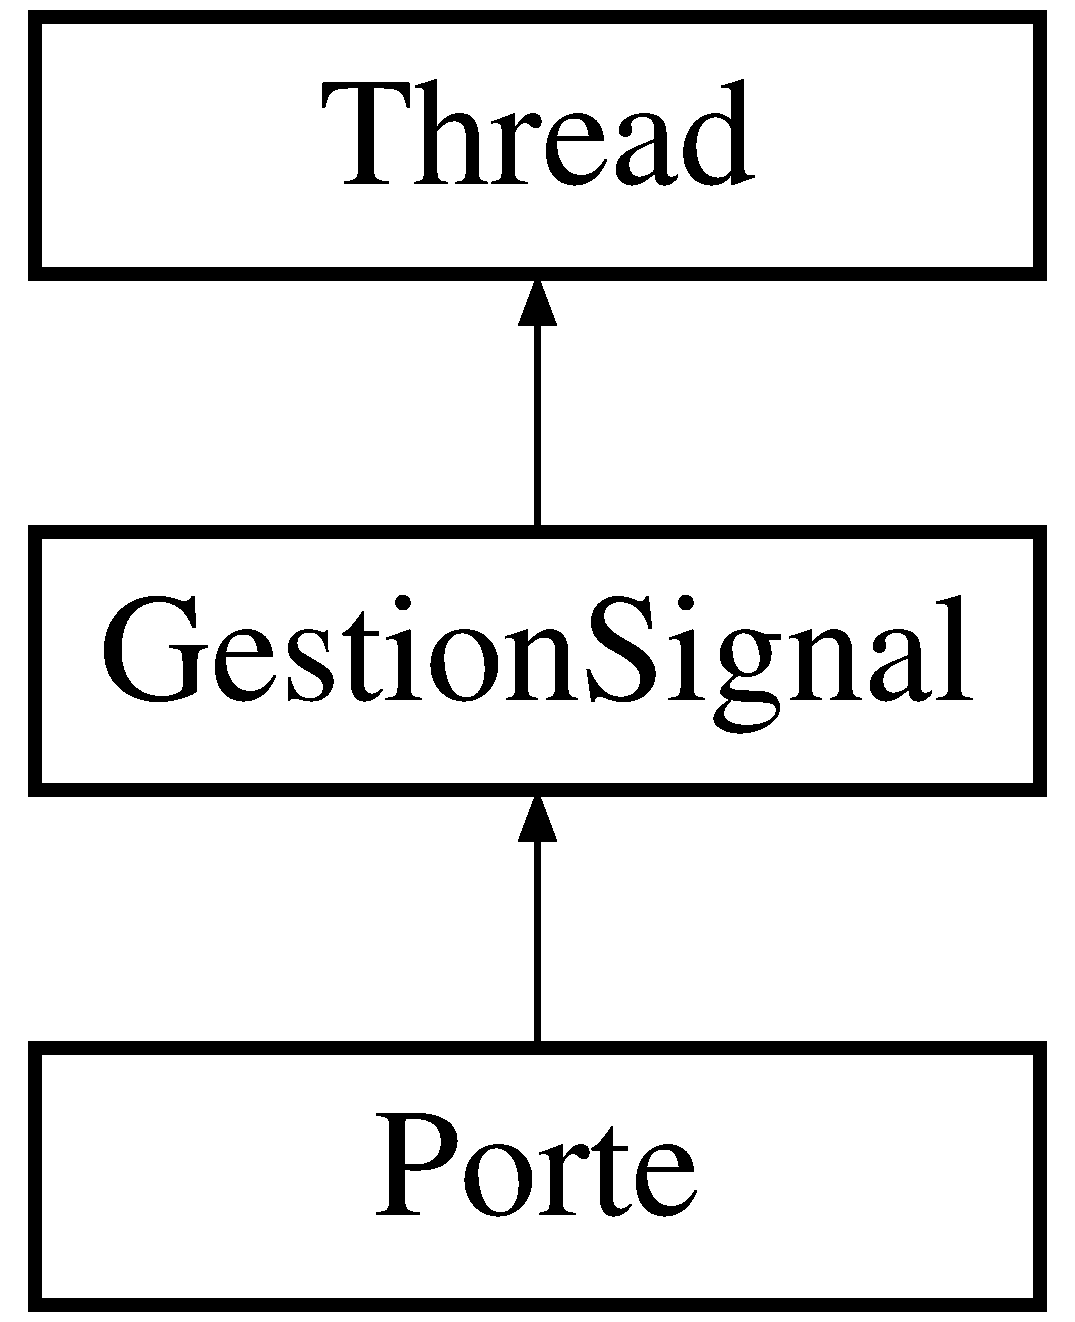
\includegraphics[height=3cm]{classPorte}
\end{center}
\end{figure}
\subsection*{Fonctions membres publiques}
\begin{DoxyCompactItemize}
\item 
\hypertarget{classPorte_a05e19e08d3ff7f043ea0a10a5014641a}{
\hyperlink{classPorte_a05e19e08d3ff7f043ea0a10a5014641a}{Porte} ()}
\label{classPorte_a05e19e08d3ff7f043ea0a10a5014641a}

\begin{DoxyCompactList}\small\item\em Constructeur d'une porte. \item\end{DoxyCompactList}\item 
\hypertarget{classPorte_a4b2871553ecea50b1aae06fff264ce4b}{
\hyperlink{classPorte_a4b2871553ecea50b1aae06fff264ce4b}{Porte} (\hyperlink{classRame}{Rame} $\ast$r)}
\label{classPorte_a4b2871553ecea50b1aae06fff264ce4b}

\begin{DoxyCompactList}\small\item\em Constructeur d'une porte. \item\end{DoxyCompactList}\item 
\hypertarget{classPorte_a7b82ccac24bfd8b7fa701f7601328d6c}{
\hyperlink{classPorte_a7b82ccac24bfd8b7fa701f7601328d6c}{$\sim$Porte} ()}
\label{classPorte_a7b82ccac24bfd8b7fa701f7601328d6c}

\begin{DoxyCompactList}\small\item\em Destructeur d'une porte. \item\end{DoxyCompactList}\item 
\hypertarget{classPorte_a6da489b2494630c2e49afb6b14135565}{
void \hyperlink{classPorte_a6da489b2494630c2e49afb6b14135565}{run} ()}
\label{classPorte_a6da489b2494630c2e49afb6b14135565}

\begin{DoxyCompactList}\small\item\em Comportement d'une porte. \item\end{DoxyCompactList}\item 
\hypertarget{classPorte_a588ea2df3d7e9db98d4ce7426c4ba7f9}{
void \hyperlink{classPorte_a588ea2df3d7e9db98d4ce7426c4ba7f9}{ouvrir} ()}
\label{classPorte_a588ea2df3d7e9db98d4ce7426c4ba7f9}

\begin{DoxyCompactList}\small\item\em Ouverture de la porte. \item\end{DoxyCompactList}\item 
\hypertarget{classPorte_a3718ae4efe9d301d94fda91040764114}{
void \hyperlink{classPorte_a3718ae4efe9d301d94fda91040764114}{fermer} ()}
\label{classPorte_a3718ae4efe9d301d94fda91040764114}

\begin{DoxyCompactList}\small\item\em Fermeture de la porte. \item\end{DoxyCompactList}\item 
\hypertarget{classPorte_aed677d56fb34ab8ed8c9beb6e338452a}{
bool \hyperlink{classPorte_aed677d56fb34ab8ed8c9beb6e338452a}{isOpen} ()}
\label{classPorte_aed677d56fb34ab8ed8c9beb6e338452a}

\begin{DoxyCompactList}\small\item\em Retourne l'etat de la porte. \item\end{DoxyCompactList}\item 
void \hyperlink{classPorte_a612d63b6b888d391ac7ab3530cb6fecb}{afficher} (QPainter $\ast$painter, int x, int y, int wPorte, int hElement)
\begin{DoxyCompactList}\small\item\em Affichage graphique d'une porte. \item\end{DoxyCompactList}\item 
\hypertarget{classPorte_a27ff96c2b4acc8d223d744ecd31aa3a3}{
void \hyperlink{classPorte_a27ff96c2b4acc8d223d744ecd31aa3a3}{demanderOuverture} ()}
\label{classPorte_a27ff96c2b4acc8d223d744ecd31aa3a3}

\begin{DoxyCompactList}\small\item\em Demande l'ouverture de la porte avant ou à l'arrivée a une station. \item\end{DoxyCompactList}\item 
virtual QString \hyperlink{classPorte_a773001136f190566b51b4e24c4323409}{getClasse} ()
\begin{DoxyCompactList}\small\item\em Retourne le nom de la classe \hyperlink{classPorte}{Porte}. \item\end{DoxyCompactList}\item 
int \hyperlink{classPorte_a65ae951c733e2741c6dcc5ef336ff7d4}{getNumPorte} ()
\begin{DoxyCompactList}\small\item\em Retourne l'identificateur de porte. \item\end{DoxyCompactList}\item 
\hypertarget{classPorte_ab87d9b41a1a6a877318da3f336392744}{
void \hyperlink{classPorte_ab87d9b41a1a6a877318da3f336392744}{createSignal} ()}
\label{classPorte_ab87d9b41a1a6a877318da3f336392744}

\begin{DoxyCompactList}\small\item\em Gestion des signaux: Signals::OuvrirPorte : signal de la rame pour autoriser l'ouverture de la porte Signals::FermerPorte : signal de la rame pour demander la fermeture de la porte. Renvoie un signal Signals::PorteFermee a la rame lorsque la porte est fermee. \item\end{DoxyCompactList}\end{DoxyCompactItemize}
\subsection*{Attributs publics statiques}
\begin{DoxyCompactItemize}
\item 
\hypertarget{classPorte_ace96ffd106c02645ae1f9e50d77f54bf}{
static int {\bfseries nombrePortes} = 0}
\label{classPorte_ace96ffd106c02645ae1f9e50d77f54bf}

\end{DoxyCompactItemize}


\subsection{Documentation des fonctions membres}
\hypertarget{classPorte_a612d63b6b888d391ac7ab3530cb6fecb}{
\index{Porte@{Porte}!afficher@{afficher}}
\index{afficher@{afficher}!Porte@{Porte}}
\subsubsection[{afficher}]{\setlength{\rightskip}{0pt plus 5cm}void Porte::afficher (QPainter $\ast$ {\em painter}, \/  int {\em x}, \/  int {\em y}, \/  int {\em wPorte}, \/  int {\em hElement})}}
\label{classPorte_a612d63b6b888d391ac7ab3530cb6fecb}


Affichage graphique d'une porte. 


\begin{DoxyParams}{Paramètres}
\item[{\em }]\end{DoxyParams}
\hypertarget{classPorte_a773001136f190566b51b4e24c4323409}{
\index{Porte@{Porte}!getClasse@{getClasse}}
\index{getClasse@{getClasse}!Porte@{Porte}}
\subsubsection[{getClasse}]{\setlength{\rightskip}{0pt plus 5cm}virtual QString Porte::getClasse ()\hspace{0.3cm}{\ttfamily  \mbox{[}inline, virtual\mbox{]}}}}
\label{classPorte_a773001136f190566b51b4e24c4323409}


Retourne le nom de la classe \hyperlink{classPorte}{Porte}. 

\begin{DoxyReturn}{Renvoie}
le nom de la classe 
\end{DoxyReturn}


Réimplémentée à partir de \hyperlink{classThread_ad055e7c603fda2607670f69c32b2d98a}{Thread}.

\hypertarget{classPorte_a65ae951c733e2741c6dcc5ef336ff7d4}{
\index{Porte@{Porte}!getNumPorte@{getNumPorte}}
\index{getNumPorte@{getNumPorte}!Porte@{Porte}}
\subsubsection[{getNumPorte}]{\setlength{\rightskip}{0pt plus 5cm}int Porte::getNumPorte ()\hspace{0.3cm}{\ttfamily  \mbox{[}inline\mbox{]}}}}
\label{classPorte_a65ae951c733e2741c6dcc5ef336ff7d4}


Retourne l'identificateur de porte. 

\begin{DoxyReturn}{Renvoie}
l'id de la porte 
\end{DoxyReturn}


La documentation de cette classe a été générée à partir des fichiers suivants :\begin{DoxyCompactItemize}
\item 
porte.h\item 
porte.cpp\end{DoxyCompactItemize}

\hypertarget{classRame}{
\section{Référence de la classe Rame}
\label{classRame}\index{Rame@{Rame}}
}
Graphe d'héritage de Rame:\begin{figure}[H]
\begin{center}
\leavevmode
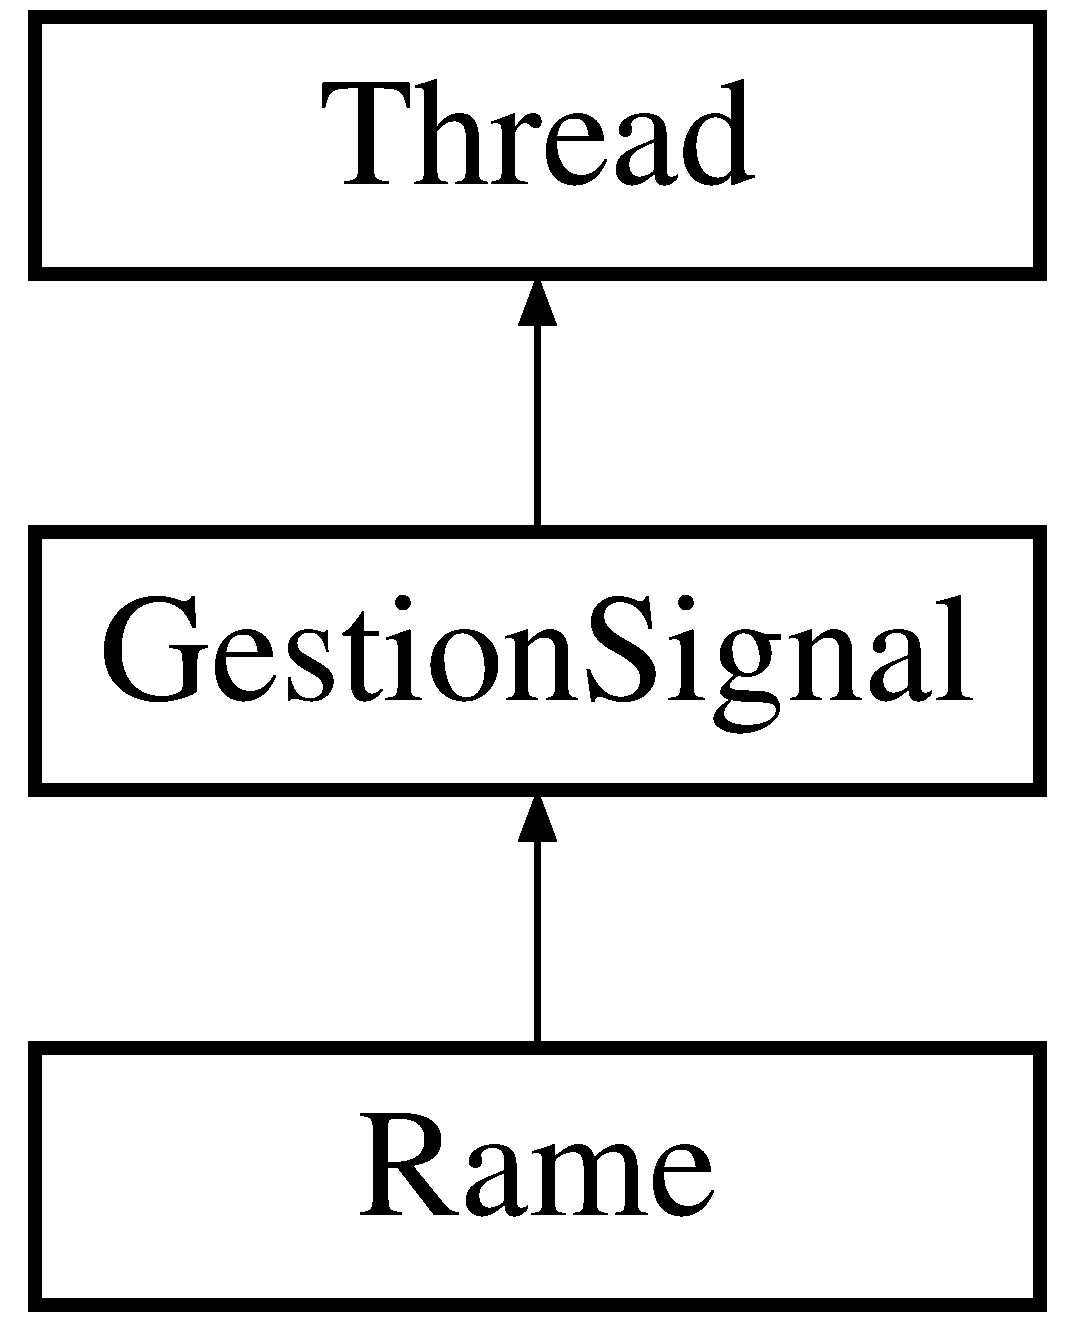
\includegraphics[height=3cm]{classRame}
\end{center}
\end{figure}
\subsection*{Types publics}
\begin{DoxyCompactItemize}
\item 
enum {\bfseries Sens} \{ {\bfseries Aller}, 
{\bfseries Retour}
 \}
\end{DoxyCompactItemize}
\subsection*{Fonctions membres publiques}
\begin{DoxyCompactItemize}
\item 
\hypertarget{classRame_adef53f3ecf010d61beaddf3b70cff9a7}{
\hyperlink{classRame_adef53f3ecf010d61beaddf3b70cff9a7}{Rame} ()}
\label{classRame_adef53f3ecf010d61beaddf3b70cff9a7}

\begin{DoxyCompactList}\small\item\em Constructeur d'une rame. \item\end{DoxyCompactList}\item 
\hyperlink{classRame_a8066c138d427e7ae1236a563cf118c9a}{Rame} (\hyperlink{classLigne}{Ligne} $\ast$)
\begin{DoxyCompactList}\small\item\em Constructeur d'une rame. \item\end{DoxyCompactList}\item 
\hypertarget{classRame_a01b0bee8b4dd0b34e264691754a09cf9}{
\hyperlink{classRame_a01b0bee8b4dd0b34e264691754a09cf9}{$\sim$Rame} ()}
\label{classRame_a01b0bee8b4dd0b34e264691754a09cf9}

\begin{DoxyCompactList}\small\item\em Destructeur d'une rame. \item\end{DoxyCompactList}\item 
\hypertarget{classRame_a795c6b2b9c2de73d65d667fa6499356b}{
void \hyperlink{classRame_a795c6b2b9c2de73d65d667fa6499356b}{run} ()}
\label{classRame_a795c6b2b9c2de73d65d667fa6499356b}

\begin{DoxyCompactList}\small\item\em Comportement d'une rame. \item\end{DoxyCompactList}\item 
void \hyperlink{classRame_ae17128baab9f80372d1a1b6cd94ca2cd}{afficher} (QPainter $\ast$painter, int x, int y, int, int)
\begin{DoxyCompactList}\small\item\em Affichage graphique d'une porte. \item\end{DoxyCompactList}\item 
\hypertarget{classRame_a967aa23c6da624b0f7b03be6613e76c6}{
void \hyperlink{classRame_a967aa23c6da624b0f7b03be6613e76c6}{avancer} ()}
\label{classRame_a967aa23c6da624b0f7b03be6613e76c6}

\begin{DoxyCompactList}\small\item\em Avance la rame d'une case. \item\end{DoxyCompactList}\item 
int \hyperlink{classRame_a69a35184fb6ae56508438c553f096dd2}{getPosition} ()
\begin{DoxyCompactList}\small\item\em Retourne la position de la rame sur la ligne. \item\end{DoxyCompactList}\item 
void \hyperlink{classRame_a2334e438ad1f3e3f93d0580f7f220411}{setPosition} (int)
\begin{DoxyCompactList}\small\item\em Modifie la position de la rame sur la ligne. \item\end{DoxyCompactList}\item 
int \hyperlink{classRame_aa37e23c49eadb05d1bb5c08a73f7b751}{getNumRame} ()
\begin{DoxyCompactList}\small\item\em Retourne l'id de la rame. \item\end{DoxyCompactList}\item 
int \hyperlink{classRame_a6a7326b0c9ea2eb2fb2954d6aa8aeabb}{getNbPassager} ()
\begin{DoxyCompactList}\small\item\em Retourne le nombre de passager. \item\end{DoxyCompactList}\item 
void \hyperlink{classRame_a8bc41267a14836e1e95cd59f5ac3def6}{monte} (QList$<$ \hyperlink{classPassager}{Passager} $\ast$ $>$ plistepassager)
\begin{DoxyCompactList}\small\item\em Faire monter un groupe de passager dans la rame. \item\end{DoxyCompactList}\item 
QList$<$ \hyperlink{classPassager}{Passager} $\ast$ $>$ \hyperlink{classRame_a1ed8e8d1cee489bead9aa2b4b0fb6ca6}{descend} (\hyperlink{classStation}{Station} $\ast$pstation)
\begin{DoxyCompactList}\small\item\em Faire descendre un groupe de passager de la rame. \item\end{DoxyCompactList}\item 
\hypertarget{classRame_aa2541afe9a8f16d929803812048a323f}{
void \hyperlink{classRame_aa2541afe9a8f16d929803812048a323f}{razListePassager} ()}
\label{classRame_aa2541afe9a8f16d929803812048a323f}

\begin{DoxyCompactList}\small\item\em Vider la liste de passager. \item\end{DoxyCompactList}\end{DoxyCompactItemize}
\subsection*{Attributs publics}
\begin{DoxyCompactItemize}
\item 
\hypertarget{classRame_a525bea4947e6fcf110902fafdd380cf8}{
Sens {\bfseries sens}}
\label{classRame_a525bea4947e6fcf110902fafdd380cf8}

\end{DoxyCompactItemize}
\subsection*{Attributs publics statiques}
\begin{DoxyCompactItemize}
\item 
\hypertarget{classRame_a55df3add73446e18b84b6fca24a191c3}{
static int {\bfseries nbRame} = 0}
\label{classRame_a55df3add73446e18b84b6fca24a191c3}

\end{DoxyCompactItemize}


\subsection{Documentation des constructeurs et destructeur}
\hypertarget{classRame_a8066c138d427e7ae1236a563cf118c9a}{
\index{Rame@{Rame}!Rame@{Rame}}
\index{Rame@{Rame}!Rame@{Rame}}
\subsubsection[{Rame}]{\setlength{\rightskip}{0pt plus 5cm}Rame::Rame ({\bf Ligne} $\ast$ {\em ligne})}}
\label{classRame_a8066c138d427e7ae1236a563cf118c9a}


Constructeur d'une rame. 


\begin{DoxyParams}{Paramètres}
\item[{\em une}]ligne \end{DoxyParams}


\subsection{Documentation des fonctions membres}
\hypertarget{classRame_ae17128baab9f80372d1a1b6cd94ca2cd}{
\index{Rame@{Rame}!afficher@{afficher}}
\index{afficher@{afficher}!Rame@{Rame}}
\subsubsection[{afficher}]{\setlength{\rightskip}{0pt plus 5cm}void Rame::afficher (QPainter $\ast$ {\em painter}, \/  int {\em x}, \/  int {\em y}, \/  int {\em wElement}, \/  int {\em hElement})}}
\label{classRame_ae17128baab9f80372d1a1b6cd94ca2cd}


Affichage graphique d'une porte. 


\begin{DoxyParams}{Paramètres}
\item[{\em }]\end{DoxyParams}
\hypertarget{classRame_a1ed8e8d1cee489bead9aa2b4b0fb6ca6}{
\index{Rame@{Rame}!descend@{descend}}
\index{descend@{descend}!Rame@{Rame}}
\subsubsection[{descend}]{\setlength{\rightskip}{0pt plus 5cm}QList$<$ {\bf Passager} $\ast$ $>$ Rame::descend ({\bf Station} $\ast$ {\em pstation})}}
\label{classRame_a1ed8e8d1cee489bead9aa2b4b0fb6ca6}


Faire descendre un groupe de passager de la rame. 


\begin{DoxyParams}{Paramètres}
\item[{\em Une}]station \end{DoxyParams}
\begin{DoxyReturn}{Renvoie}
Un groupe de passager 
\end{DoxyReturn}
\hypertarget{classRame_a6a7326b0c9ea2eb2fb2954d6aa8aeabb}{
\index{Rame@{Rame}!getNbPassager@{getNbPassager}}
\index{getNbPassager@{getNbPassager}!Rame@{Rame}}
\subsubsection[{getNbPassager}]{\setlength{\rightskip}{0pt plus 5cm}int Rame::getNbPassager ()}}
\label{classRame_a6a7326b0c9ea2eb2fb2954d6aa8aeabb}


Retourne le nombre de passager. 

\begin{DoxyReturn}{Renvoie}
nombre de passager 
\end{DoxyReturn}
\hypertarget{classRame_aa37e23c49eadb05d1bb5c08a73f7b751}{
\index{Rame@{Rame}!getNumRame@{getNumRame}}
\index{getNumRame@{getNumRame}!Rame@{Rame}}
\subsubsection[{getNumRame}]{\setlength{\rightskip}{0pt plus 5cm}int Rame::getNumRame ()}}
\label{classRame_aa37e23c49eadb05d1bb5c08a73f7b751}


Retourne l'id de la rame. 

\begin{DoxyReturn}{Renvoie}
id d'une rame 
\end{DoxyReturn}
\hypertarget{classRame_a69a35184fb6ae56508438c553f096dd2}{
\index{Rame@{Rame}!getPosition@{getPosition}}
\index{getPosition@{getPosition}!Rame@{Rame}}
\subsubsection[{getPosition}]{\setlength{\rightskip}{0pt plus 5cm}int Rame::getPosition ()}}
\label{classRame_a69a35184fb6ae56508438c553f096dd2}


Retourne la position de la rame sur la ligne. 

\begin{DoxyReturn}{Renvoie}
la position de la rame 
\end{DoxyReturn}
\hypertarget{classRame_a8bc41267a14836e1e95cd59f5ac3def6}{
\index{Rame@{Rame}!monte@{monte}}
\index{monte@{monte}!Rame@{Rame}}
\subsubsection[{monte}]{\setlength{\rightskip}{0pt plus 5cm}void Rame::monte (QList$<$ {\bf Passager} $\ast$ $>$ {\em plistepassager})}}
\label{classRame_a8bc41267a14836e1e95cd59f5ac3def6}


Faire monter un groupe de passager dans la rame. 


\begin{DoxyParams}{Paramètres}
\item[{\em Liste}]de passager \end{DoxyParams}
\hypertarget{classRame_a2334e438ad1f3e3f93d0580f7f220411}{
\index{Rame@{Rame}!setPosition@{setPosition}}
\index{setPosition@{setPosition}!Rame@{Rame}}
\subsubsection[{setPosition}]{\setlength{\rightskip}{0pt plus 5cm}void Rame::setPosition (int {\em i})}}
\label{classRame_a2334e438ad1f3e3f93d0580f7f220411}


Modifie la position de la rame sur la ligne. 


\begin{DoxyParams}{Paramètres}
\item[{\em une}]position \end{DoxyParams}


La documentation de cette classe a été générée à partir des fichiers suivants :\begin{DoxyCompactItemize}
\item 
rame.h\item 
rame.cpp\end{DoxyCompactItemize}

\hypertarget{classSignals}{
\section{Référence de la classe Signals}
\label{classSignals}\index{Signals@{Signals}}
}
\subsection*{Types publics}
\begin{DoxyCompactItemize}
\item 
enum {\bfseries TypeSignal} \{ \par
{\bfseries Demande}, 
{\bfseries EstPasse}, 
{\bfseries Arret}, 
{\bfseries Passe}, 
\par
{\bfseries OuvrirPorte}, 
{\bfseries FermerPorte}, 
{\bfseries PorteFermee}
 \}
\end{DoxyCompactItemize}
\subsection*{Fonctions membres publiques}
\begin{DoxyCompactItemize}
\item 
\hypertarget{classSignals_abb20260e11bbaf3cdfc45cbc6506349a}{
\hyperlink{classSignals_abb20260e11bbaf3cdfc45cbc6506349a}{Signals} (\hyperlink{classGestionSignal}{GestionSignal} $\ast$, TypeSignal)}
\label{classSignals_abb20260e11bbaf3cdfc45cbc6506349a}

\begin{DoxyCompactList}\small\item\em constructeur de Signal. \item\end{DoxyCompactList}\item 
\hypertarget{classSignals_a023cdc52c51b2d8c33e0af2714b4cb04}{
\hyperlink{classSignals_a023cdc52c51b2d8c33e0af2714b4cb04}{$\sim$Signals} ()}
\label{classSignals_a023cdc52c51b2d8c33e0af2714b4cb04}

\begin{DoxyCompactList}\small\item\em Destructeur de Feu. \item\end{DoxyCompactList}\item 
\hyperlink{classGestionSignal}{GestionSignal} $\ast$ \hyperlink{classSignals_abd873414eef1e8deb5dc8bcae33aa8fe}{emetteur} ()
\begin{DoxyCompactList}\small\item\em Retourne l'emetteur du signal. \item\end{DoxyCompactList}\item 
void \hyperlink{classSignals_a8a58cb7d36939d77e0319e47e787f262}{setEmetteur} (\hyperlink{classGestionSignal}{GestionSignal} $\ast$)
\begin{DoxyCompactList}\small\item\em Definir l'emetteur du signal. \item\end{DoxyCompactList}\item 
TypeSignal \hyperlink{classSignals_af14716654fb552b8940935694edc1b69}{type} ()
\begin{DoxyCompactList}\small\item\em Retourne le type du signal. \item\end{DoxyCompactList}\end{DoxyCompactItemize}


\subsection{Documentation des fonctions membres}
\hypertarget{classSignals_abd873414eef1e8deb5dc8bcae33aa8fe}{
\index{Signals@{Signals}!emetteur@{emetteur}}
\index{emetteur@{emetteur}!Signals@{Signals}}
\subsubsection[{emetteur}]{\setlength{\rightskip}{0pt plus 5cm}{\bf GestionSignal} $\ast$ Signals::emetteur ()}}
\label{classSignals_abd873414eef1e8deb5dc8bcae33aa8fe}


Retourne l'emetteur du signal. 

\begin{DoxyReturn}{Renvoie}
signal emetteur 
\end{DoxyReturn}
\hypertarget{classSignals_a8a58cb7d36939d77e0319e47e787f262}{
\index{Signals@{Signals}!setEmetteur@{setEmetteur}}
\index{setEmetteur@{setEmetteur}!Signals@{Signals}}
\subsubsection[{setEmetteur}]{\setlength{\rightskip}{0pt plus 5cm}void Signals::setEmetteur ({\bf GestionSignal} $\ast$ {\em e})}}
\label{classSignals_a8a58cb7d36939d77e0319e47e787f262}


Definir l'emetteur du signal. 


\begin{DoxyParams}{Paramètres}
\item[{\em signal}]emetteur \end{DoxyParams}
\hypertarget{classSignals_af14716654fb552b8940935694edc1b69}{
\index{Signals@{Signals}!type@{type}}
\index{type@{type}!Signals@{Signals}}
\subsubsection[{type}]{\setlength{\rightskip}{0pt plus 5cm}Signals::TypeSignal Signals::type ()}}
\label{classSignals_af14716654fb552b8940935694edc1b69}


Retourne le type du signal. 

\begin{DoxyReturn}{Renvoie}
type du signal 
\end{DoxyReturn}


La documentation de cette classe a été générée à partir des fichiers suivants :\begin{DoxyCompactItemize}
\item 
signals.h\item 
signals.cpp\end{DoxyCompactItemize}

\hypertarget{classStation}{
\section{Référence de la classe Station}
\label{classStation}\index{Station@{Station}}
}
Graphe d'héritage de Station:\begin{figure}[H]
\begin{center}
\leavevmode
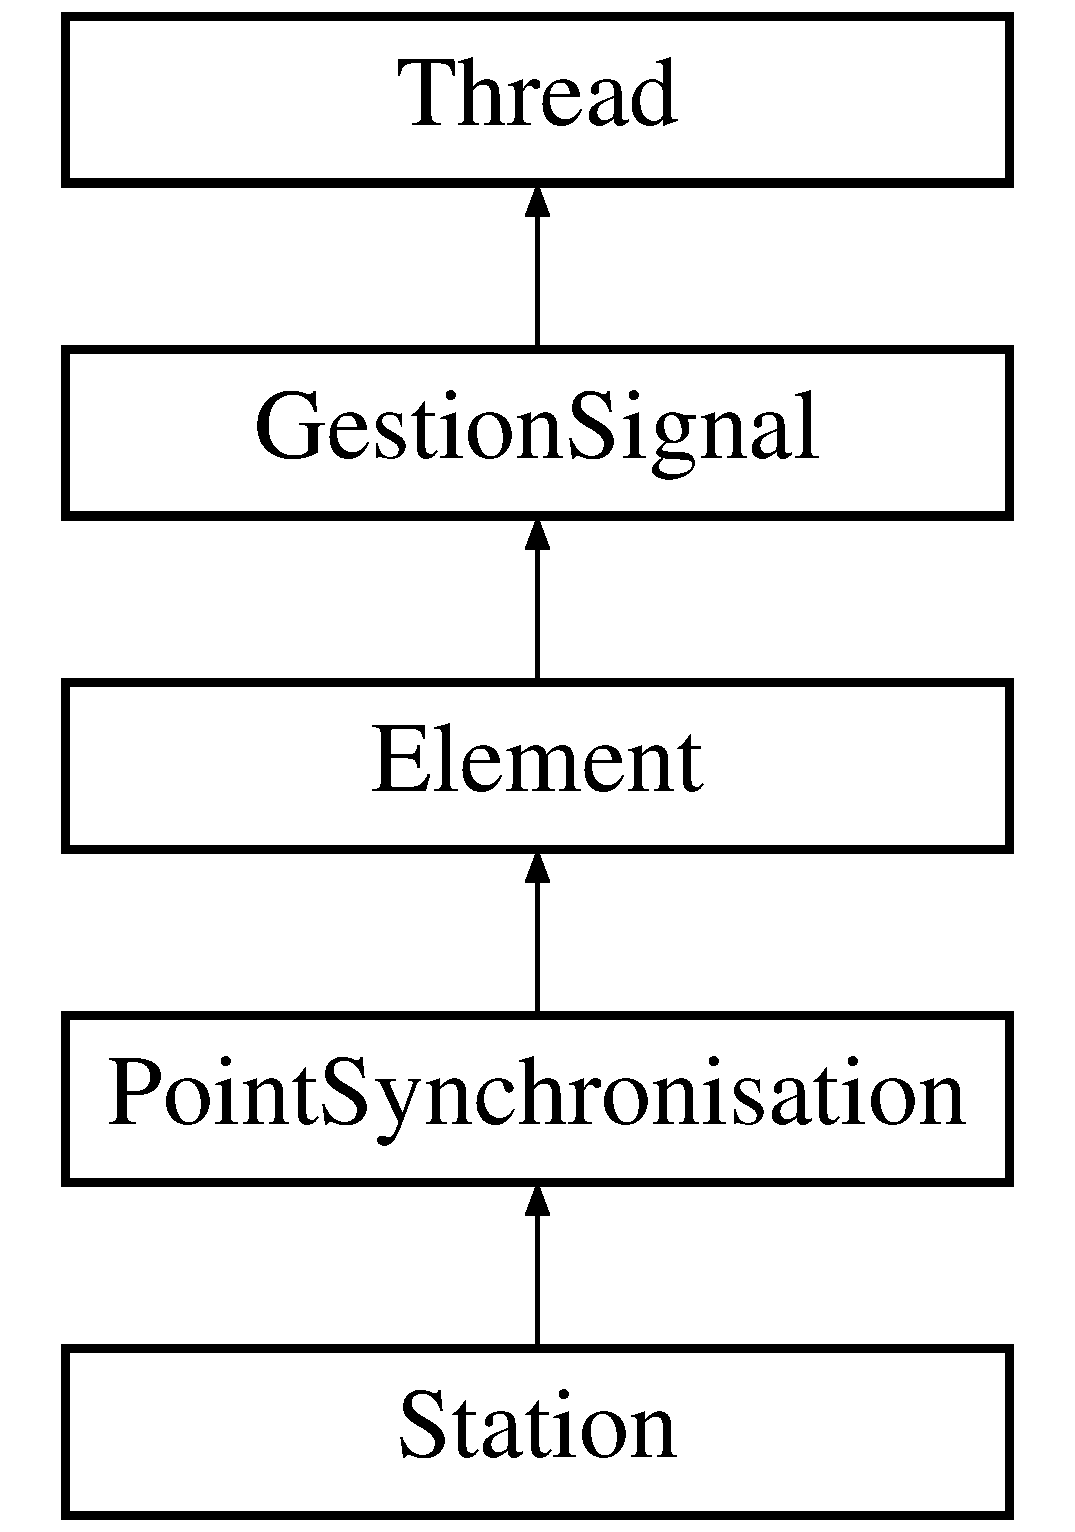
\includegraphics[height=5cm]{classStation}
\end{center}
\end{figure}
\subsection*{Types publics}
\begin{DoxyCompactItemize}
\item 
enum {\bfseries Type} \{ {\bfseries Terminus}, 
{\bfseries Intermediaire}
 \}
\end{DoxyCompactItemize}
\subsection*{Fonctions membres publiques}
\begin{DoxyCompactItemize}
\item 
\hypertarget{classStation_a73d335726aad1d844d81cda6d9fd74e6}{
\hyperlink{classStation_a73d335726aad1d844d81cda6d9fd74e6}{Station} ()}
\label{classStation_a73d335726aad1d844d81cda6d9fd74e6}

\begin{DoxyCompactList}\small\item\em constructeur de \hyperlink{classStation}{Station}. \item\end{DoxyCompactList}\item 
\hyperlink{classStation_a3f359a7bed774082d2f1b5927ce4dd5c}{Station} (QString nomLigne, Station::Type, \hyperlink{classLigne}{Ligne} $\ast$)
\begin{DoxyCompactList}\small\item\em constructeur de \hyperlink{classStation}{Station}. \item\end{DoxyCompactList}\item 
void \hyperlink{classStation_aa4918eec32fe4f3484f629564b84e160}{afficher} (QPainter $\ast$painter, int x, int y, int, int, bool)
\begin{DoxyCompactList}\small\item\em Affichage graphique d'une station. \item\end{DoxyCompactList}\item 
virtual QString \hyperlink{classStation_aea030824145267b81a453f5b56227cae}{getClasse} ()
\begin{DoxyCompactList}\small\item\em Retourne le nom de la classe \hyperlink{classStation}{Station}. \item\end{DoxyCompactList}\item 
\hypertarget{classStation_a73c0d1c00b8de39ff4eb16be708e9a92}{
void \hyperlink{classStation_a73c0d1c00b8de39ff4eb16be708e9a92}{run} ()}
\label{classStation_a73c0d1c00b8de39ff4eb16be708e9a92}

\begin{DoxyCompactList}\small\item\em Comportement d'une station. \item\end{DoxyCompactList}\item 
QString \hyperlink{classStation_ac73e2b60d199734b494e84fa065a6643}{getNom} ()
\begin{DoxyCompactList}\small\item\em Retourne le nom de la station. \item\end{DoxyCompactList}\item 
\hyperlink{classLigne}{Ligne} $\ast$ \hyperlink{classStation_a3ee72b5920d69350770fa056d6b675bc}{getLigne} ()
\begin{DoxyCompactList}\small\item\em Retourne ligne de la station. \item\end{DoxyCompactList}\item 
void \hyperlink{classStation_a41ad1728246bbecd645a7a9679a2e59c}{createSignal} ()
\item 
bool \hyperlink{classStation_ad2c82ba6d816f24c26970c4468351807}{estTerminus} ()
\begin{DoxyCompactList}\small\item\em Verifie le type de station. \item\end{DoxyCompactList}\item 
\hypertarget{classStation_a81ea74879cf784be7f89153be99be03d}{
void \hyperlink{classStation_a81ea74879cf784be7f89153be99be03d}{setPassagers} ()}
\label{classStation_a81ea74879cf784be7f89153be99be03d}

\begin{DoxyCompactList}\small\item\em Ajoute des passager en attente a la station. \item\end{DoxyCompactList}\end{DoxyCompactItemize}
\subsection*{Attributs publics statiques}
\begin{DoxyCompactItemize}
\item 
\hypertarget{classStation_a0735f4fa937dd9018dedb764c3a2ee49}{
static int {\bfseries nombreStations} = 0}
\label{classStation_a0735f4fa937dd9018dedb764c3a2ee49}

\end{DoxyCompactItemize}


\subsection{Documentation des constructeurs et destructeur}
\hypertarget{classStation_a3f359a7bed774082d2f1b5927ce4dd5c}{
\index{Station@{Station}!Station@{Station}}
\index{Station@{Station}!Station@{Station}}
\subsubsection[{Station}]{\setlength{\rightskip}{0pt plus 5cm}Station::Station (QString {\em nomLigne}, \/  Station::Type {\em t}, \/  {\bf Ligne} $\ast$ {\em pligne})}}
\label{classStation_a3f359a7bed774082d2f1b5927ce4dd5c}


constructeur de \hyperlink{classStation}{Station}. 


\begin{DoxyParams}{Paramètres}
\item[{\em nom}]de la ligne \item[{\em type}]de station \item[{\em une}]ligne \end{DoxyParams}


\subsection{Documentation des fonctions membres}
\hypertarget{classStation_aa4918eec32fe4f3484f629564b84e160}{
\index{Station@{Station}!afficher@{afficher}}
\index{afficher@{afficher}!Station@{Station}}
\subsubsection[{afficher}]{\setlength{\rightskip}{0pt plus 5cm}void Station::afficher (QPainter $\ast$ {\em painter}, \/  int {\em x}, \/  int {\em y}, \/  int {\em wElement}, \/  int {\em hElement}, \/  bool {\em affNom})}}
\label{classStation_aa4918eec32fe4f3484f629564b84e160}


Affichage graphique d'une station. 


\begin{DoxyParams}{Paramètres}
\item[{\em }]\end{DoxyParams}
\hypertarget{classStation_a41ad1728246bbecd645a7a9679a2e59c}{
\index{Station@{Station}!createSignal@{createSignal}}
\index{createSignal@{createSignal}!Station@{Station}}
\subsubsection[{createSignal}]{\setlength{\rightskip}{0pt plus 5cm}void Station::createSignal ()\hspace{0.3cm}{\ttfamily  \mbox{[}virtual\mbox{]}}}}
\label{classStation_a41ad1728246bbecd645a7a9679a2e59c}
Gestion des signaux recus: Signals::Demande Signals::EstPasse : indique que la rame est partie, remet le feu a rouge. 

Réimplémentée à partir de \hyperlink{classElement_a4f4cc97e3122305ec6f4a8953aba23d5}{Element}.

\hypertarget{classStation_ad2c82ba6d816f24c26970c4468351807}{
\index{Station@{Station}!estTerminus@{estTerminus}}
\index{estTerminus@{estTerminus}!Station@{Station}}
\subsubsection[{estTerminus}]{\setlength{\rightskip}{0pt plus 5cm}bool Station::estTerminus ()}}
\label{classStation_ad2c82ba6d816f24c26970c4468351807}


Verifie le type de station. 

\begin{DoxyReturn}{Renvoie}
station terminus = 1 sinon 0 
\end{DoxyReturn}
\hypertarget{classStation_aea030824145267b81a453f5b56227cae}{
\index{Station@{Station}!getClasse@{getClasse}}
\index{getClasse@{getClasse}!Station@{Station}}
\subsubsection[{getClasse}]{\setlength{\rightskip}{0pt plus 5cm}virtual QString Station::getClasse ()\hspace{0.3cm}{\ttfamily  \mbox{[}inline, virtual\mbox{]}}}}
\label{classStation_aea030824145267b81a453f5b56227cae}


Retourne le nom de la classe \hyperlink{classStation}{Station}. 

\begin{DoxyReturn}{Renvoie}
le nom de la classe 
\end{DoxyReturn}


Réimplémentée à partir de \hyperlink{classThread_ad055e7c603fda2607670f69c32b2d98a}{Thread}.

\hypertarget{classStation_a3ee72b5920d69350770fa056d6b675bc}{
\index{Station@{Station}!getLigne@{getLigne}}
\index{getLigne@{getLigne}!Station@{Station}}
\subsubsection[{getLigne}]{\setlength{\rightskip}{0pt plus 5cm}{\bf Ligne} $\ast$ Station::getLigne ()}}
\label{classStation_a3ee72b5920d69350770fa056d6b675bc}


Retourne ligne de la station. 

\begin{DoxyReturn}{Renvoie}
la ligne de la station 
\end{DoxyReturn}
\hypertarget{classStation_ac73e2b60d199734b494e84fa065a6643}{
\index{Station@{Station}!getNom@{getNom}}
\index{getNom@{getNom}!Station@{Station}}
\subsubsection[{getNom}]{\setlength{\rightskip}{0pt plus 5cm}QString Station::getNom ()}}
\label{classStation_ac73e2b60d199734b494e84fa065a6643}


Retourne le nom de la station. 

\begin{DoxyReturn}{Renvoie}
le nom de la station 
\end{DoxyReturn}


La documentation de cette classe a été générée à partir des fichiers suivants :\begin{DoxyCompactItemize}
\item 
station.h\item 
station.cpp\end{DoxyCompactItemize}

\hypertarget{classThread}{
\section{Référence de la classe Thread}
\label{classThread}\index{Thread@{Thread}}
}
Graphe d'héritage de Thread:\begin{figure}[H]
\begin{center}
\leavevmode
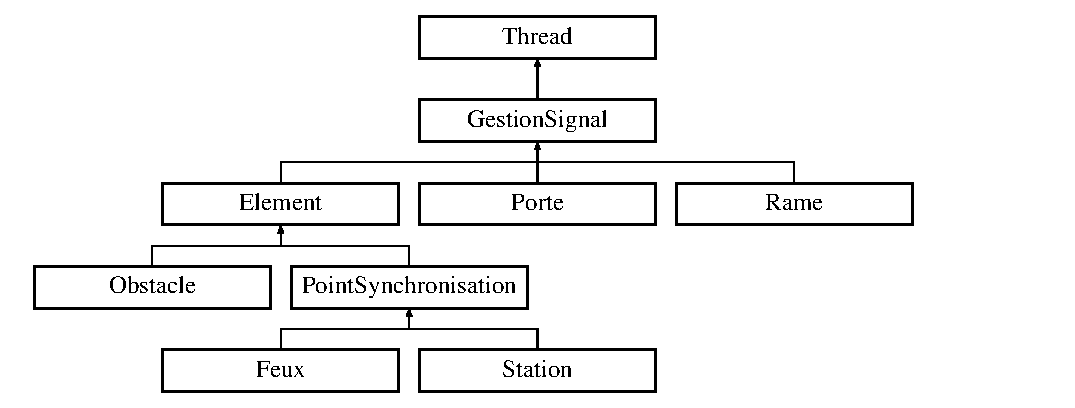
\includegraphics[height=5cm]{classThread}
\end{center}
\end{figure}
\subsection*{Fonctions membres publiques}
\begin{DoxyCompactItemize}
\item 
\hypertarget{classThread_a95c703fb8f2f27cb64f475a8c940864a}{
\hyperlink{classThread_a95c703fb8f2f27cb64f475a8c940864a}{Thread} ()}
\label{classThread_a95c703fb8f2f27cb64f475a8c940864a}

\begin{DoxyCompactList}\small\item\em constructeur de \hyperlink{classThread}{Thread}. \item\end{DoxyCompactList}\item 
\hypertarget{classThread_a37d9edd3a1a776cbc27dedff949c9726}{
virtual \hyperlink{classThread_a37d9edd3a1a776cbc27dedff949c9726}{$\sim$Thread} ()}
\label{classThread_a37d9edd3a1a776cbc27dedff949c9726}

\begin{DoxyCompactList}\small\item\em Destructeur de \hyperlink{classThread}{Thread}. \item\end{DoxyCompactList}\item 
\hypertarget{classThread_aae90dfabab3e1776cf01a26e7ee3a620}{
virtual void \hyperlink{classThread_aae90dfabab3e1776cf01a26e7ee3a620}{run} ()=0}
\label{classThread_aae90dfabab3e1776cf01a26e7ee3a620}

\begin{DoxyCompactList}\small\item\em Comportement d'un \hyperlink{classThread}{Thread}. \item\end{DoxyCompactList}\item 
\hypertarget{classThread_a1f53ee62bd30a7924186ef26150ce262}{
virtual void \hyperlink{classThread_a1f53ee62bd30a7924186ef26150ce262}{start} ()}
\label{classThread_a1f53ee62bd30a7924186ef26150ce262}

\begin{DoxyCompactList}\small\item\em Demarrage d'un thread. \item\end{DoxyCompactList}\item 
\hypertarget{classThread_a4d9d788e98388a3217831a9046709deb}{
virtual void \hyperlink{classThread_a4d9d788e98388a3217831a9046709deb}{join} ()}
\label{classThread_a4d9d788e98388a3217831a9046709deb}

\begin{DoxyCompactList}\small\item\em Attente du join. \item\end{DoxyCompactList}\item 
\hypertarget{classThread_abd50159ecd409936f454c2321f673616}{
virtual void \hyperlink{classThread_abd50159ecd409936f454c2321f673616}{stop} ()}
\label{classThread_abd50159ecd409936f454c2321f673616}

\begin{DoxyCompactList}\small\item\em Arret du \hyperlink{classThread}{Thread}. \item\end{DoxyCompactList}\item 
virtual QString \hyperlink{classThread_ad055e7c603fda2607670f69c32b2d98a}{getClasse} ()
\begin{DoxyCompactList}\small\item\em Retourne le nom de la classe \hyperlink{classThread}{Thread}. \item\end{DoxyCompactList}\item 
pthread\_\-t \hyperlink{classThread_a2bcb649ad0f9304744c18e5c15d7fa8e}{id} ()
\begin{DoxyCompactList}\small\item\em Retourne l'id du thread. \item\end{DoxyCompactList}\item 
bool \hyperlink{classThread_a06a3cea9c644b36becc3dc21444d9f99}{getEtatThread} ()
\begin{DoxyCompactList}\small\item\em Retourne l'etat du thread. \item\end{DoxyCompactList}\end{DoxyCompactItemize}
\subsection*{Amis}
\begin{DoxyCompactItemize}
\item 
\hypertarget{classThread_ab6e610ca1cdc02783d947d3341c17ddf}{
void $\ast$ \hyperlink{classThread_ab6e610ca1cdc02783d947d3341c17ddf}{start\_\-thread} (void $\ast$)}
\label{classThread_ab6e610ca1cdc02783d947d3341c17ddf}

\begin{DoxyCompactList}\small\item\em Fonction lancee lors de la creation d'un thread. \item\end{DoxyCompactList}\end{DoxyCompactItemize}


\subsection{Documentation des fonctions membres}
\hypertarget{classThread_ad055e7c603fda2607670f69c32b2d98a}{
\index{Thread@{Thread}!getClasse@{getClasse}}
\index{getClasse@{getClasse}!Thread@{Thread}}
\subsubsection[{getClasse}]{\setlength{\rightskip}{0pt plus 5cm}virtual QString Thread::getClasse ()\hspace{0.3cm}{\ttfamily  \mbox{[}inline, virtual\mbox{]}}}}
\label{classThread_ad055e7c603fda2607670f69c32b2d98a}


Retourne le nom de la classe \hyperlink{classThread}{Thread}. 

\begin{DoxyReturn}{Renvoie}
le nom de la classe 
\end{DoxyReturn}


Réimplémentée dans \hyperlink{classFeux_ac06b420ea2bb015007eb03ca2401176e}{Feux}, \hyperlink{classObstacle_a7773466eaafb92cef0ec22f5cc79522c}{Obstacle}, \hyperlink{classPorte_a773001136f190566b51b4e24c4323409}{Porte}, et \hyperlink{classStation_aea030824145267b81a453f5b56227cae}{Station}.

\hypertarget{classThread_a06a3cea9c644b36becc3dc21444d9f99}{
\index{Thread@{Thread}!getEtatThread@{getEtatThread}}
\index{getEtatThread@{getEtatThread}!Thread@{Thread}}
\subsubsection[{getEtatThread}]{\setlength{\rightskip}{0pt plus 5cm}bool Thread::getEtatThread ()}}
\label{classThread_a06a3cea9c644b36becc3dc21444d9f99}


Retourne l'etat du thread. 

\begin{DoxyReturn}{Renvoie}
etat du thread ACTIF=1 
\end{DoxyReturn}
\hypertarget{classThread_a2bcb649ad0f9304744c18e5c15d7fa8e}{
\index{Thread@{Thread}!id@{id}}
\index{id@{id}!Thread@{Thread}}
\subsubsection[{id}]{\setlength{\rightskip}{0pt plus 5cm}pthread\_\-t Thread::id ()}}
\label{classThread_a2bcb649ad0f9304744c18e5c15d7fa8e}


Retourne l'id du thread. 

\begin{DoxyReturn}{Renvoie}
id du thread 
\end{DoxyReturn}


La documentation de cette classe a été générée à partir des fichiers suivants :\begin{DoxyCompactItemize}
\item 
thread.h\item 
thread.cpp\end{DoxyCompactItemize}

\printindex
\end{document}
